%\documentclass[]{article}
%\usepackage{lmodern}
%\usepackage{amssymb,amsmath}
%\usepackage{ifxetex,ifluatex}
%\usepackage{fixltx2e} % provides \textsubscript
%\ifnum 0\ifxetex 1\fi\ifluatex 1\fi=0 % if pdftex
%  \usepackage[T1]{fontenc}
%  \usepackage[utf8]{inputenc}
%\else % if luatex or xelatex
%  \ifxetex
%    \usepackage{mathspec}
%  \else
%    \usepackage{fontspec}
%  \fi
%  \defaultfontfeatures{Ligatures=TeX,Scale=MatchLowercase}
%\fi
%% use upquote if available, for straight quotes in verbatim environments
%\IfFileExists{upquote.sty}{\usepackage{upquote}}{}
%% use microtype if available
%\IfFileExists{microtype.sty}{%
%\usepackage[]{microtype}
%\UseMicrotypeSet[protrusion]{basicmath} % disable protrusion for tt fonts
%}{}
%\PassOptionsToPackage{hyphens}{url} % url is loaded by hyperref
%\usepackage[unicode=true]{hyperref}
%\hypersetup{
%            pdfborder={0 0 0},
%            breaklinks=true}
%\urlstyle{same}  % don't use monospace font for urls
%\usepackage{longtable,booktabs}
%% Fix footnotes in tables (requires footnote package)
%\IfFileExists{footnote.sty}{\usepackage{footnote}\makesavenoteenv{long table}}{}
%\usepackage{graphicx,grffile}
%\makeatletter
%\def\maxwidth{\ifdim\Gin@nat@width>\linewidth\linewidth\else\Gin@nat@width\fi}
%\def\maxheight{\ifdim\Gin@nat@height>\textheight\textheight\else\Gin@nat@height\fi}
%\makeatother
%% Scale images if necessary, so that they will not overflow the page
%% margins by default, and it is still possible to overwrite the defaults
%% using explicit options in \includegraphics[width, height, ...]{}
%\setkeys{Gin}{width=\maxwidth,height=\maxheight,keepaspectratio}
%\IfFileExists{parskip.sty}{%
%\usepackage{parskip}
%}{% else
%\setlength{\parindent}{0pt}
%\setlength{\parskip}{6pt plus 2pt minus 1pt}
%}
%\setlength{\emergencystretch}{3em}  % prevent overfull lines
%\providecommand{\tightlist}{%
%  \setlength{\itemsep}{0pt}\setlength{\parskip}{0pt}}
%\setcounter{secnumdepth}{0}
%% Redefines (sub)paragraphs to behave more like sections
%\ifx\paragraph\undefined\else
%\let\oldparagraph\paragraph
%\renewcommand{\paragraph}[1]{\oldparagraph{#1}\mbox{}}
%\fi
%\ifx\subparagraph\undefined\else
%\let\oldsubparagraph\subparagraph
%\renewcommand{\subparagraph}[1]{\oldsubparagraph{#1}\mbox{}}
%\fi
%
%% set default figure placement to htbp
%\makeatletter
%\def\fps@figure{htbp}
%\makeatother
%
%
%\date{}
%
%\begin{document}
Ailing Tong\textsuperscript{1}, John T. Petroff II\textsuperscript{1},
Fong-Fu Hsu\textsuperscript{2}, Philipp A. M.
Schmidpeter\textsuperscript{3}, Crina M. Nimigean\textsuperscript{3},
Liam Sharp\textsuperscript{4}, Grace Brannigan\textsuperscript{4,5},
Wayland W. L. Cheng\textsuperscript{1,}*

From the Departments of \textsuperscript{1}Anesthesiology, and
\textsuperscript{2}Internal Medicine, Mass Spectrometry Resource,
Division of Endocrinology, Diabetes, Metabolism, and Lipid Research,
Washington University in St. Louis, MO, USA,
\textsuperscript{3}Departments of Anesthesiology, and Physiology and
Biophysics, Weill Cornell Medicine, NY, USA, and the
\textsuperscript{4}Center for Computational and Integrative Biology and
\textsuperscript{5}Department of Physics, Rutgers University, Camden,
NJ, USA.

*To whom correspondence should be addressed: Professor Wayland W. L.
Cheng, Department of Anesthesiology, Washington University School of
Medicine, Campus Box 8054, St. Louis, MO 63110. Telephone:
(314)273-7958; E-mail: wayland.cheng@wustl.edu

\section{Abstract}

Pentameric ligand-gated ion channels (pLGICs) are essential determinants
of synaptic transmission, and are modulated by specific lipids including
anionic phospholipids. The exact modulatory effect of anionic
phospholipids in pLGICs and the mechanism of this effect are not well
understood. Using native mass spectrometry, coarse-grained molecular
dynamics simulations and functional assays, we show that the anionic
phospholipid, 1-palmitoyl-2-oleoyl-phosphatidylglycerol (POPG),
preferentially binds to and stabilizes the pLGIC, Erwinia ligand-gated
ion channel (ELIC), and decreases ELIC desensitization. Mutations of
five arginines located in the interfacial regions of the transmembrane
domain (TMD) reduce POPG binding, and a subset of these mutations
increase ELIC desensitization. In contrast, the L240A mutant increases
POPG binding and decreases ELIC desensitization. The results support a
mechanism by which POPG stabilizes the open state of ELIC relative to
the desensitized state by direct binding at specific sites.

\section{Introduction}

Pentameric ligand-gated ion channels (pLGICs) are essential determinants
of synaptic transmission, and the targets of many allosteric modulators
including general anesthetics and anti-epileptics (1). These ion
channels are embedded in a heterogeneous and dynamic lipid environment
(2), and the presence of specific lipids fine-tunes the function of
pLGICs and may play a role in regulating neuronal excitability and drug
sensitivity (3-5). One nearly ubiquitous example is that of anionic
phospholipids, which are known to modulate pentameric ligand-gated ion
channels (pLGICs) such as the nicotinic acetylcholine receptor (nAchR)
(6), as well as inward rectifying potassium channels (7), K(2P) channels
(8), voltage-gated potassium channels (9, 10), and cyclic
nucleotide-gated channels (11). In pLGICs, anionic phospholipids have
been shown to shift the conformational equilibrium of the channel from
an uncoupled or desensitized state to a resting state, in which agonist
binding is effectively coupled to channel activation (12-14).

Studies of lipid modulation of ion channel function including modulation
of pLGICs have focused on two central questions: 1) what is the exact
effect of the lipid on channel function and structure, and 2) is the
effect attributable to direct binding of the lipid at specific sites?
\emph{Torpedo} nAchR channel activity measured from flux assays (6, 15,
16) and agonist-induced conformational changes (13, 17) depend on
anionic phospholipids. However, few studies have employed fast solution
changes to measure current responses of pLGICs in model membranes (18),
which is necessary to distinguish the effect of lipids on channel
gating, specifically transitions between resting, open and desensitized
states. With regard to lipid binding, early studies using electron
paramagnetic resonance (EPR) of spin-labeled lipids or lipid-induced
modification of fluorescent probes revealed an immobilized layer of
lipids surrounding nAchRs that is enriched for certain phospholipids
(19, 20) with lipids occupying specific sites (21, 22). These approaches
are, however, an indirect means to examine lipid binding to ion
channels. More recently, crystal structures of the pLGIC, Gloeobacter
ligand-gated ion channel (GLIC), revealed bound, co-purified
phospholipids in a putative open structure, and the absence of one of
these phospholipids in a locally-closed structure (23, 24). Similarly, a
putative desensitized structure of GLIC with a bound polyunsaturated
fatty acid showed loss of the aforementioned phospholipid density that
is bound to the open state (25). Both of these studies suggest that
bound phospholipids at specific sites stabilize the open state of the
channel, although the identity of these lipids remains unknown.
Furthermore, the absence of a lipid density in a crystal structure is
not necessarily an indication of lack of binding.

Native mass spectrometry (MS) has proven to be a powerful tool to
directly measure binding of endogenous and exogenous lipids to membrane
proteins (26, 27), although this approach has yet to be used to examine
pLGIC-lipid interactions. In addition, coarse-grained molecular dynamics
(MD) simulations provide a complementary approach to examine lipid
interactions with membrane-embedded pLGICs at time scales that allow
equilibration of lipid binding sites (28, 29). We sought to determine
whether phospholipids bind directly and selectively to a pLGIC by native
MS and coarse-grained MD simulations, and whether specific binding
interactions modulate channel function by patch-clamp recordings and
stopped-flow ion flux measurements from liposomes of defined lipid
composition. Erwinia ligand-gated ion channel (ELIC), a prototypical
pLGIC and biochemically tractable target, is also sensitive to its lipid
environment. ELIC was found to be inactive when reconstituted in
1-palmitoyl-2-oleoyl-phosphatidylcholine (POPC) membranes fused to
\emph{Xenopus} oocyte membranes, similar to the nAchR (30). After
optimizing native MS for ELIC, we demonstrate that phospholipids
directly bind to ELIC, with more binding observed for the anionic
phospholipid, POPG compared to zwitterionic phospholipids,
1-palmitoyl-2-oleoyl-phosphatidylethanolamine (POPE) and POPC.
Consistent with this finding, coarse-grained simulations of ELIC in a
lipid bilayer show enrichment of annular POPG compared to POPC or POPE
phospholipids. In addition, POPG selectively stabilizes ELIC against
thermal denaturation indicative of a specific binding interaction, and
reduces channel desensitization. Mutations of five arginines at the
transmembrane domain (TMD) intracellular and extracellular interfaces
decrease PG binding while a subset of these mutations increase
desensitization. Likewise, the L240A mutant, which reduces
desensitization, increases PG binding. The results support the
long-standing hypothesis that anionic phospholipids stabilize the open
state of pLGICs by direct binding to sites in the TMD adjacent to the
lipid-facing transmembrane helix 4 (TM4) (3).

\section{Results}

\subsection{Selective binding of phospholipids to ELIC}

\begin{figure}
\center
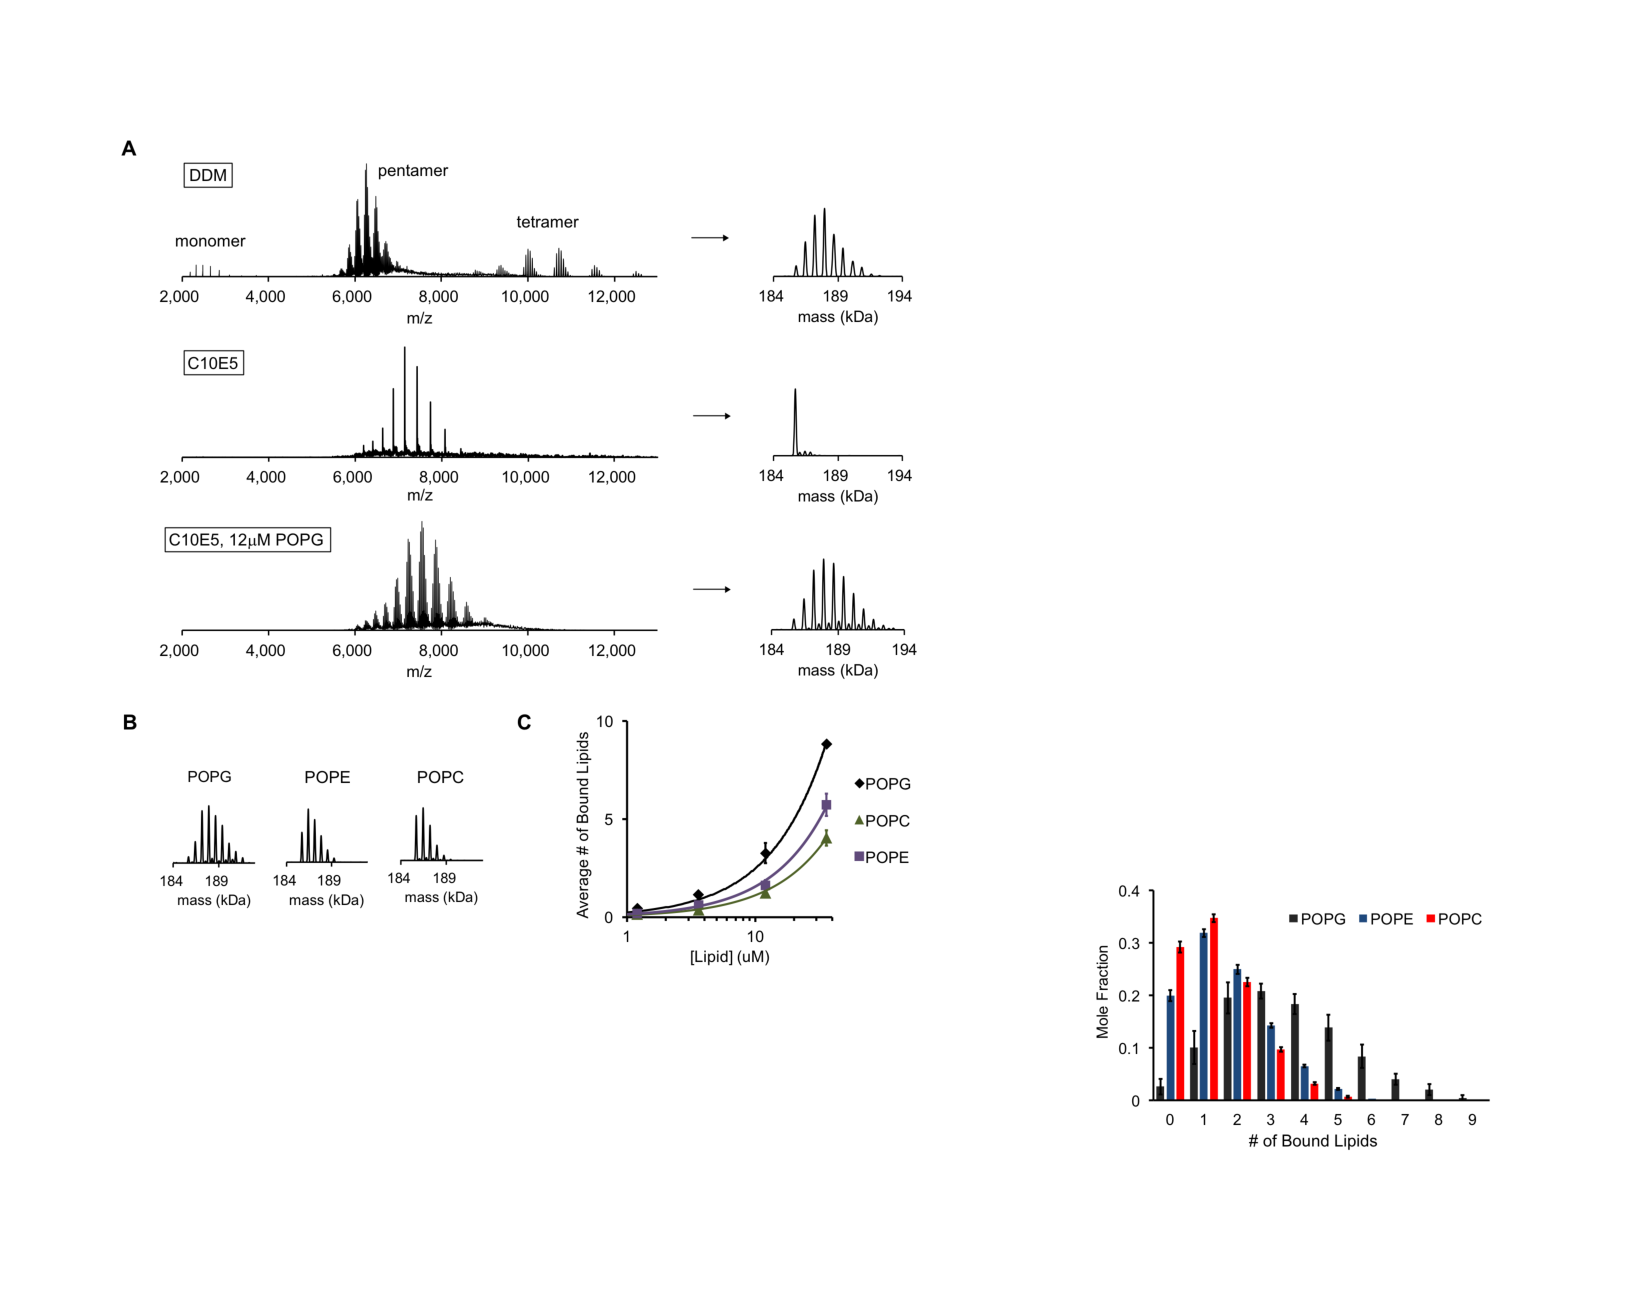
\includegraphics[width=\linewidth]{./pandoc_test/media/image1.pdf}
	\begin{flushleft}

\caption[POPG binds selectively to ELIC.] {POPG binds selectively to ELIC. (A) Native MS spectra of ELIC in DDM, C10E5, and C10E5 with 12 $\mu$M POPG. Left shows full spectra and right shows deconvoluted spectra. (B) Deconvoluted spectra of ELIC in 12 $\mu$M of the indicated phospholipid. (C) Plot of the average number of bound phospholipids per pentamer at varying concentrations of POPG, POPE and POPC (n=3-6, $\pm$SD). Data are fit to a sigmoid binding curve.}
	\label{fig:one}
	\end{flushleft}

\end{figure}

Native MS of ELIC purified in dodecyl maltoside (DDM) was optimized on a
Q-Exactive EMR mass spectrometer as previously described (27). Optimal
desolvation of the pentamer required activation energies that resulted
in some dissociation into tetramer and monomer (Fig. \ref{fig:one}A). Nevertheless,
both the pentamer and tetramer species showed multiple bound small
molecules of \textasciitilde{}750 Da, likely corresponding to
co-purified phospholipids (up to 8 and 6 lipids per multimer were
observed for the pentamer and tetramer, respectively) (Fig. \ref{fig:one}A). To
determine the identity of these lipids, we performed a lipid extraction
from the purified ELIC preparation, and analyzed the sample using tandem
MS. This revealed multiple PE and PG phospholipids with different acyl
chains that mirror the phospholipids extracted from \emph{E. coli}
membranes (Table \ref{tab:Supplementary Table 1}). Quantification of the MS intensities
for PG relative to PE species yielded a higher relative abundance of PG
co-purified with ELIC compared to \emph{E. coli} membranes, suggesting
that ELIC preferentially binds PG in its native environment
(Fig. \ref{fig:Supplementary Fig. 1}, Table \ref{tab:Supplementary Table 1}).

\begin{figure}
\center
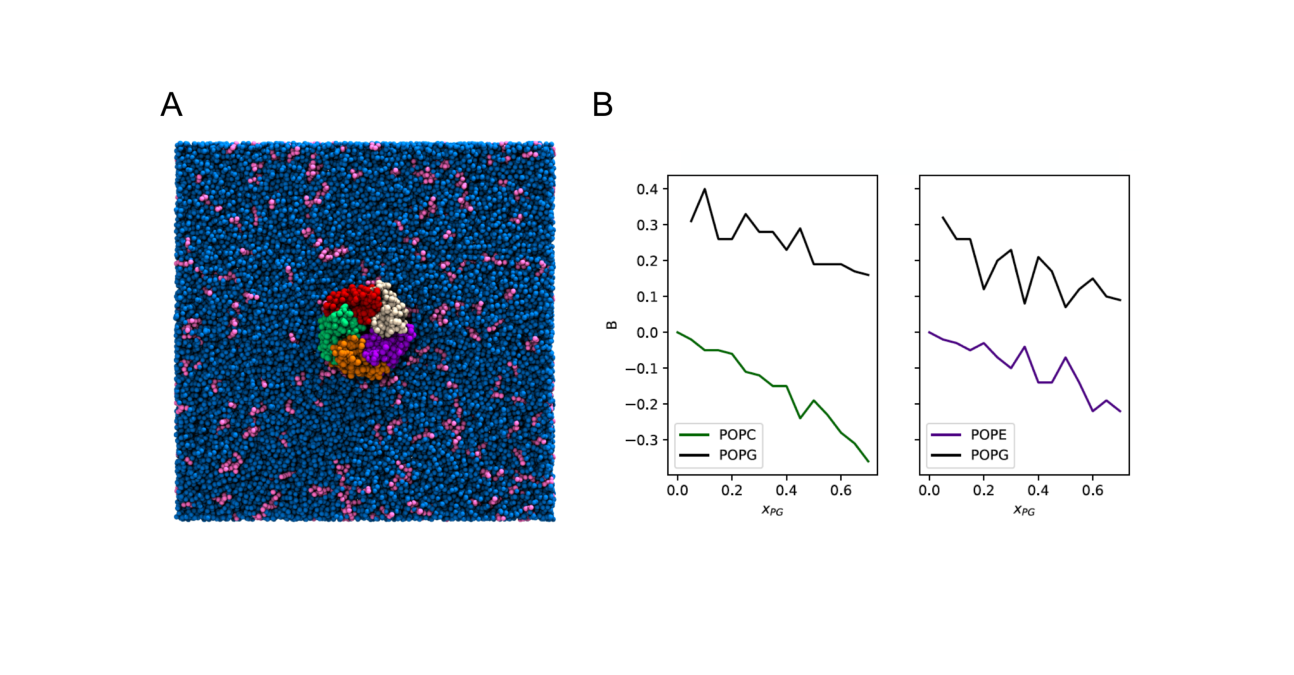
\includegraphics[width=\linewidth]{./pandoc_test/media/image2.pdf}
	\begin{flushleft}

\caption[Enrichment of POPG among ELIC boundary phospholipids from coarse-grained simulations.] {Enrichment of POPG among ELIC boundary phospholipids from coarse-grained simulations. (A) Image of the simulation model of ELIC embedded in a membrane consisting of $10\%$ POPG (pink) and $90\%$ POPC (blue). The view is from the extracellular side of ELIC perpendicular to the membrane. (B) The boundary enrichment metric, B, is shown for phospholipid species in POPC/POPG membranes (left) or POPE/POPG membranes (right) over a range of POPG mole fractions $(x_{PG})$. B is defined in Equation 4.3 (see Methods) and reflects the fractional difference between the amount of a lipid species found in the boundary and the bulk membrane: B$>$0 indicates enrichment, B$<$0 indicates depletion, and B$=$0 indicates no difference in mole fraction between the bulk and the boundary.}  \label{fig:two}
	\end{flushleft}

\end{figure}

To examine direct binding of exogenous phospholipids to ELIC, we performed
a detergent screen to delipidate ELIC focusing on detergents that are
also superior for native MS measurements (31). The polyethylene
glycol-based detergent, C10E5, proved best for this application,
yielding a stable, delipidated pentamer by native MS with lower charge
states and no dissociation of the pentamer (Fig. \ref{fig:one}A). This observation
is consistent with previous reports for this detergent in other membrane
proteins (31, 32). Addition of varying concentrations of the anionic
phospholipid, POPG, to 1 $\mu$M ELIC showed concentration dependent binding
(Fig. \ref{fig:Supplementary Fig. 2}). We quantified this binding by calculating the
average number of bound phospholipids at each concentration. For
example, at 12 $\mu$M POPG, native MS spectra revealed up to 9 bound POPG
and an average of 2.9 POPG per pentamer (Fig. \ref{fig:one}B and 1C). The average
number of bound POPG was equivalent for most charge states, and
decreased modestly at charge states higher than +26 likely due to
electrostatic repulsion within the ELIC-POPG complexes (Fig. \ref{fig:Supplementary
Fig. 3}); therefore, deconvolution was performed for charge states +26
and lower. Less binding was observed for the neutral phospholipids, POPE
and POPC (Fig. \ref{fig:one}B and 1C), indicating that the anionic phospholipid,
POPG, either binds with higher affinity or at a greater number of sites.

To further examine phospholipid interactions with ELIC using a molecular
model, coarse-grained MD simulations were performed on binary POPG/POPC
and POPG/POPE model membranes containing a single ELIC pentamer (Fig.
\ref{fig:two} A). Unlike fully-atomistic simulations, coarse-grained simulations
permit significant diffusion of lipids over simulation time scales. The
boundary lipid composition can thus equilibrate over the simulation
time, even if it varies significantly from the bulk membrane
composition. The POPG fraction was varied between 0 and 70\%. Enrichment
or depletion of POPG among boundary lipids for each concentration was
quantified using the boundary lipid metric B (Equation 4.3, see Methods).
For a given lipid species, B\textgreater{}0 reflects enrichment, B
\textless{} 0 reflects depletion, and B=0 reflects random mixing. For
POPG, B\textgreater{}0 for all compositions tested (Fig. \ref{fig:two}B). This
result indicates that if POPG is present in the membrane, it is enriched
among boundary lipids. This enrichment is strongest for lower amounts of
POPG (i.e. lower \(x_{\text{POPG}}\)), consistent with specific binding
of POPG to ELIC.

The average number of boundary phospholipids was 31.6 $\pm$ 2.5 across all
compositions, and the total did not vary systematically with membrane
composition. Assuming, therefore, that the stoichiometries of binding
for these phospholipids to ELIC are similar, we fit the native MS
binding data for each phospholipid to a binomial distribution binding
model that assumes 32 binding sites of equivalent affinity (see
Methods). While this is an oversimplification of phospholipid binding to
ELIC in a membrane, it provides a reasonable approximation to the MS
data, and reveals that POPG binds to ELIC with \textasciitilde{}1.9x and
2.8x higher affinity than POPE and POPC, respectively (Fig. \ref{fig:Supplementary
Fig. 4}). Overall, we conclude that POPG binds to ELIC with higher
affinity than POPE or POPC, resulting in POPG enrichment of annular
phospholipids as seen in the coarse-grained MD simulations.

\subsection{Selective effect of POPG on ELIC stability and function}

To determine the effect of POPG binding on ELIC, we first tested the
stability of purified, delipidated ELIC in C10E5 against thermal
denaturation in the absence and presence of POPG (33). ELIC was heated
to a temperature that resulted in 85\% decrease in the amplitude of the
pentamer peak as assessed by size exclusion chromatography (32
\textsuperscript{o}C for 15 min). POPG significantly increased the
thermal stability of 1 $\mu$M ELIC with an EC\textsubscript{50}
(concentration of POPG for 50\% effect) of 52 $\mu$M (Fig. \ref{fig:four}A). The thermal
stabilizing effect of a phospholipid was defined as the ratio of the
pentamer peak height after heating with lipid versus no lipid. In
contrast, POPE and POPC had no effect on ELIC stability (Fig. \ref{fig:four}A),
indicating that POPG binding selectively stabilizes the structure of
ELIC. Having performed our POPG binding experiment and thermal stability
assay under the same conditions, it is possible to relate the average
number of bound POPG to its stabilizing effect. 36 $\mu$M POPG was the
highest concentration for which the average number of bound POPG could
be determined due to the overlapping of charge states from lipid-bound
species (Fig.\ref{fig:one}A, Fig. \ref{fig:Supplementary Fig. 2}). Although POPG binding does not
approach saturation at this concentration, extrapolation of POPG binding
and relating this extrapolation to the thermal stabilizing effect
provides an approximation of the number of bound POPG needed to
stabilize ELIC against thermal denaturation. Supplementary Figure 5
shows a relationship between the number of bound POPG and the
stabilizing effect, which was derived by equating the POPG concentration
from the functions of POPG binding (Fig. \ref{fig:one}C) and thermal stability data
(Fig. \ref{fig:four}A). The relationship estimates that 32 POPG (number of annular
lipids in ELIC from MD simulations) yields \textasciitilde{}82\% of the
thermal stabilizing effect (Fig. \ref{fig:Supplementary Fig. 5}).

Next, we assessed the effect of POPG on ELIC function by reconstituting
the channel in giant liposomes. Optimal formation of giant liposomes was
achieved using a 2:1:1 ratio of POPC:POPE:POPG (i.e. 25 mole\% POPG). In
this lipid membrane composition, robust ELIC currents were elicited with
excised patch-clamp recordings using the agonist, cysteamine, with a
peak dose response EC\textsubscript{50} of 5.1 mM (Fig. \ref{fig:four}B, Fig. \ref{fig:three},
Fig. \ref{fig:Supplementary Fig. 6}A). Patch-clamp recordings were performed with 0.5
mM BaCl\textsubscript{2} in the pipette and bath, which is predicted to
result in an increase in the EC\textsubscript{50} of cysteamine response
(34). Near saturating currents were achieved at 30 mM cysteamine at
which ELIC activated and desensitized with time constants of 134 ms and
1.9 s, respectively (Fig. \ref{fig:four}C and 3D,  Fig. \ref{fig:three}, Fig. \ref{fig:Supplementary Fig. 6}B).
These values are comparable to previous reports of outside-out
patch-clamp recordings in HEK cells or oocytes (35, 36). ELIC
desensitization showed complex kinetics where the majority of recordings
were best fit with a double exponential and some by a single
exponential. To combine data from all traces, weighted average time
constants from double exponential fits were averaged with time constants
from single exponential fits. The extent of desensitization was examined
by measuring currents after 20 s of cysteamine application. To examine
the effect of POPG on ELIC gating, excised patch-clamp recordings were
performed in liposomes containing 12\%, 25\%, and 40\% POPG. Increasing
the mole\% of POPG had no significant effect on cysteamine
EC\textsubscript{50} values or activation kinetics (Fig. \ref{fig:four}B, Fig. \ref{fig:three},
Fig. \ref{fig:Supplementary Fig. 6}), but reduced the rate and extent of
desensitization (Fig. \ref{fig:four}C and  \ref{fig:four}D,  Fig. \ref{fig:three}).

To examine ELIC activity in the absence of POPG, a fluorescence-based
stopped-flow flux assay was performed (37). ELIC was reconstituted into
either POPC-alone or 2:1:1 POPC:POPE:POPG liposomes encapsulating the
fluorophore ANTS (8-Aminonaphthalene-1,3,6-Trisulfonic acid). In a first
mixing step, liposomes were incubated with 5 mM cysteamine to activate
the channel for different amounts of time (10 ms to 25 s) after which a
second mixing step was performed with Tl\textsuperscript{+} containing
buffer. Tl\textsuperscript{+} can permeate through activated channels
into the liposome and thus quenches ANTS fluorescence. The quenching
kinetics are a measure of the channel activity upon cysteamine exposure
for defined incubation times (Fig. \ref{fig:four}E). In POPC liposomes, ELIC showed
less cysteamine-elicited ion flux compared to ELIC in POPC:POPE:POPG
liposomes (Fig. \ref{fig:four}E and \ref{fig:four}F, Table 4.1), as estimated from the overall rate
of Tl\textsuperscript{+} flux. The rate of activation was modestly
faster in POPC:POPE:POPG liposomes compared to POPC (Fig. \ref{fig:four}F, Table 4.1).
More strikingly, the rate of desensitization was greater than 20-fold
faster in POPC liposomes, leading to a decrease in the lifetime of the
open state (Fig. \ref{fig:four}E and \ref{fig:four}F, Table 4.1).

In summary, POPG selectively increases the thermal stability of ELIC,
and modulates channel activity by stabilizing the open relative to the
desensitized state. We hypothesize that POPG decreases receptor
desensitization by direct binding at specific sites.

\begin{figure*}
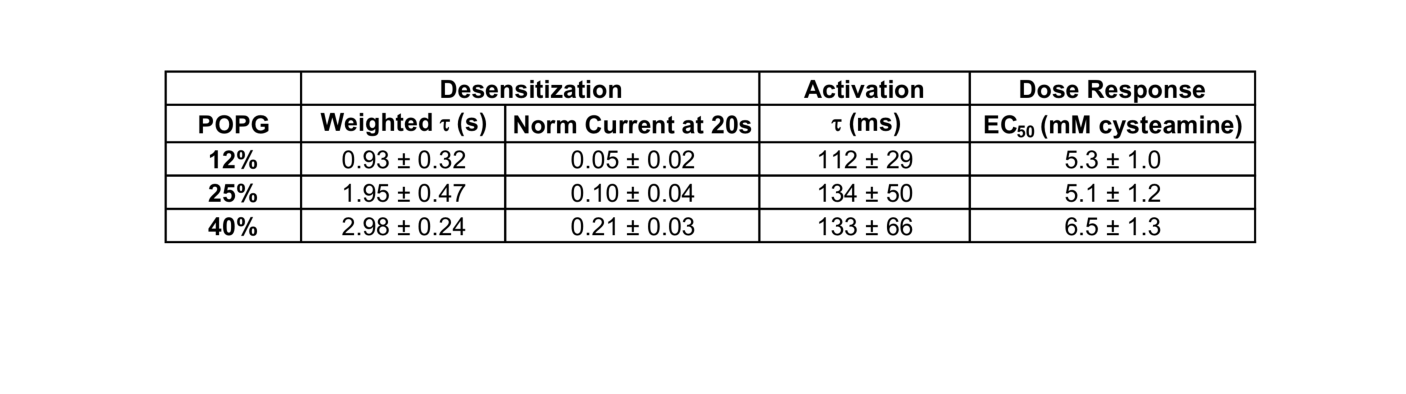
\includegraphics[width=\linewidth]{./pandoc_test/media/image3.pdf}
\caption[ELIC WT channel properties in giant liposomes composed of varying mole\% POPG (n=3-5, $\pm$SD).] {ELIC WT channel properties in giant liposomes composed of varying mole\% POPG (n=3-5, $\pm$SD). The rate and extent of desensitization are reported as weighted time constants ($\tau$), and the current after 20 s of 30 mM cysteamine application normalized to peak response. Also shown are activation time constants ($\tau$) in response to 30 mM cysteamine and EC50s for cysteamine activation.} \label{fig:three}
\end{figure*}

\begin{table}
    \caption{ELIC WT activation and desensitization rate constants derived from a double exponential fit to the time course of flux in Fig. \ref{fig:four}F (n=3, $\pm$SD). }
    \begin{tabular}{|c|c|c|}
	\hline
    {} & Activation Rate Constant & Desensitization RateConstant\\ \hline
    POPC & 24 $\pm$ 8 s\textsuperscript{-1} & 2.4 $\pm$ 0.08
    s\textsuperscript{-1}\\ \hline
    POPC:POPE:POPG (2:1:1) & 75 $\pm$ 22 s\textsuperscript{-1} & 0.11 $\pm$
    0.04 s\textsuperscript{-1}\\ \hline
    
    \end{tabular}
\end{table}


\begin{figure*}
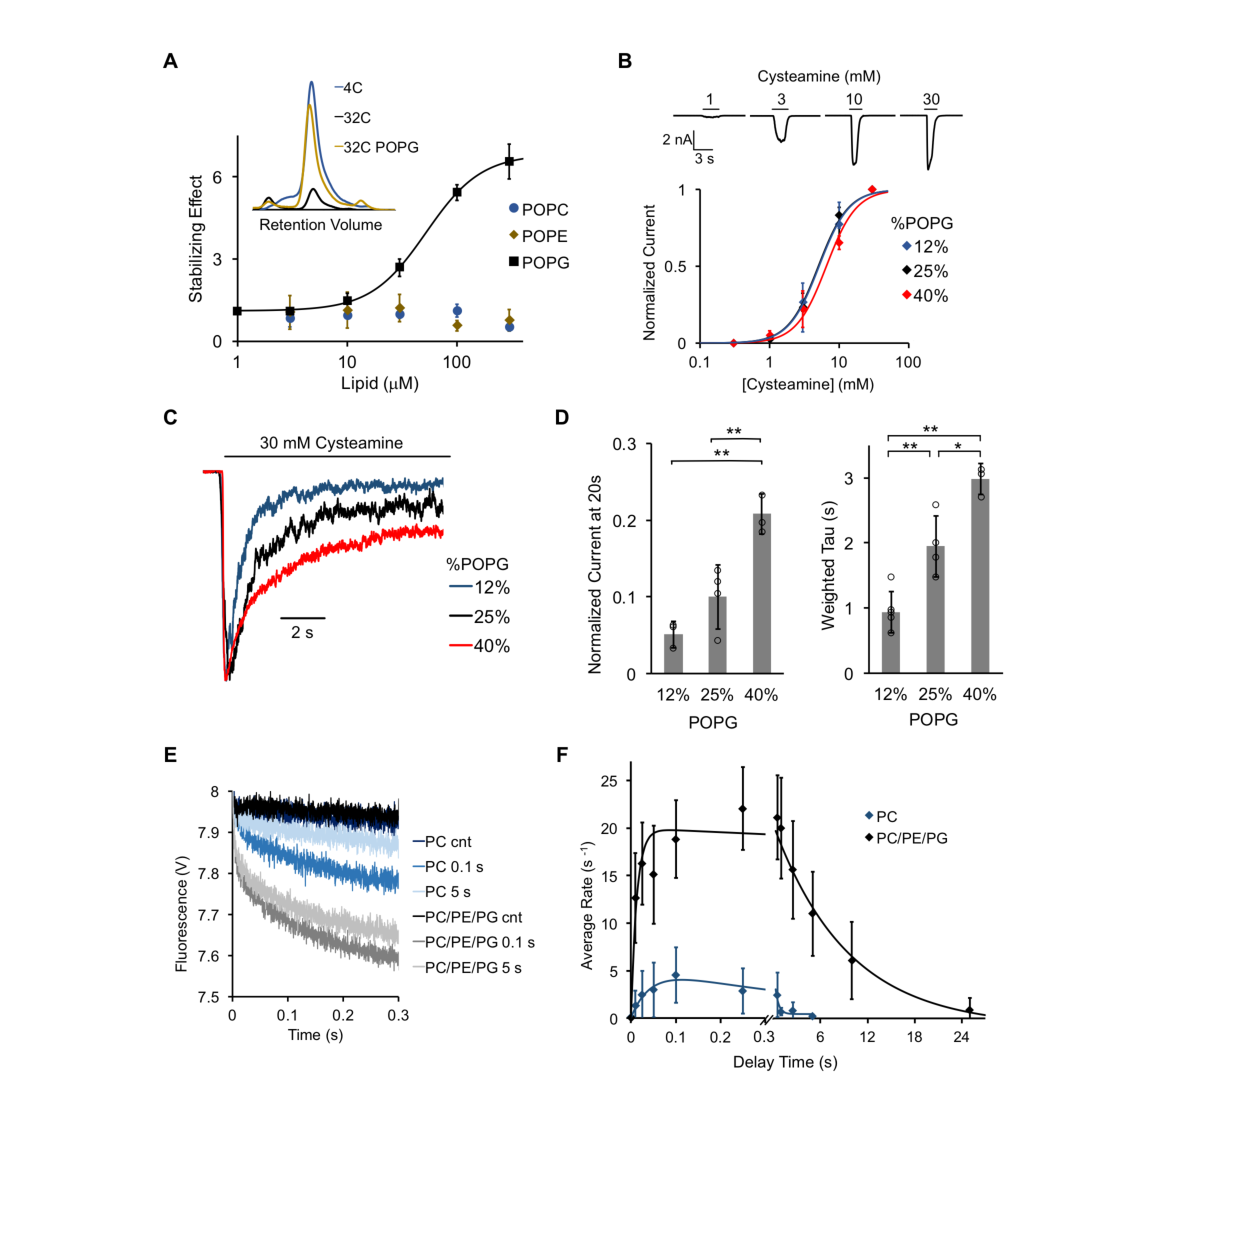
\includegraphics[width=\linewidth]{./pandoc_test/media/image4.pdf} 
\caption[POPG selectively thermally stabilizes ELIC and decreases ELIC desensitization.]{POPG selectively thermally stabilizes ELIC and decreases ELIC desensitization. Continued on the next page.}
\label{fig:four}
\end{figure*}

\begin{figure*}   
\caption[POPG selectively thermally stabilizes ELIC and decreases ELIC desensitization.] {POPG selectively thermally stabilizes ELIC and decreases ELIC desensitization. (A) Plot of stabilizing effect (defined as the ELIC pentamer peak height with phospholipid relative to control after heating) versus phospholipid concentration (n=3, $\pm$SD; EC50 = 52 $\mu$M, Hill n = 1.7). Inset shows size exclusion chromatography (SEC) profile in absorbance units of the ELIC pentamer treated at 4$^o$C, 32$^o$C, and 32$^o$C with 100 $\mu$M POPG. (B) Top: Representative ELIC current responses to 30 mM cysteamine in 25 mole\% POPG liposomes. Bottom: Normalized plots of peak current responses of ELIC to cysteamine in giant liposomes with varying mole\% POPG (n=3-5, $\pm$SD). Data are fit to Hill equation with n=2. (C) Representative ELIC currents in response to 30 mM cysteamine in liposomes with varying mole\% POPG. (D) Left: ELIC currents 20 s after application of 30 mM cysteamine normalized to peak response at varying mole\% POPG (n=4-5, $\pm$SD, **p$<$0.01). Right: Weighted tau (time constants) of ELIC desensitization at varying mole\% POPG (n=3-5, $\pm$ SD, **p$<$0.01, *p$<$0.05). (E) Representative fluorescence-quench time courses from sequential mixing stopped-flow experiments of ELIC in POPC liposomes or 2:1:1 POPC:POPE:POPG liposomes. Proteoliposomes were mixed with no cysteamine (cnt) or 5 mM cysteamine with a 0.1 or 5 s delay prior to mixing with Tl+. Note that the control traces are superimposed. (F) Rate constants extracted from quench kinetics as shown in (E) as a function of the incubation time with cysteamine. Data are fit with a double exponential yielding activation and desensitization time constants (n=3, $\pm$SD).} \label{fig:im4}
\end{figure*}


\subsection{Five interfacial arginines contribute to POPG binding}

\begin{figure*}
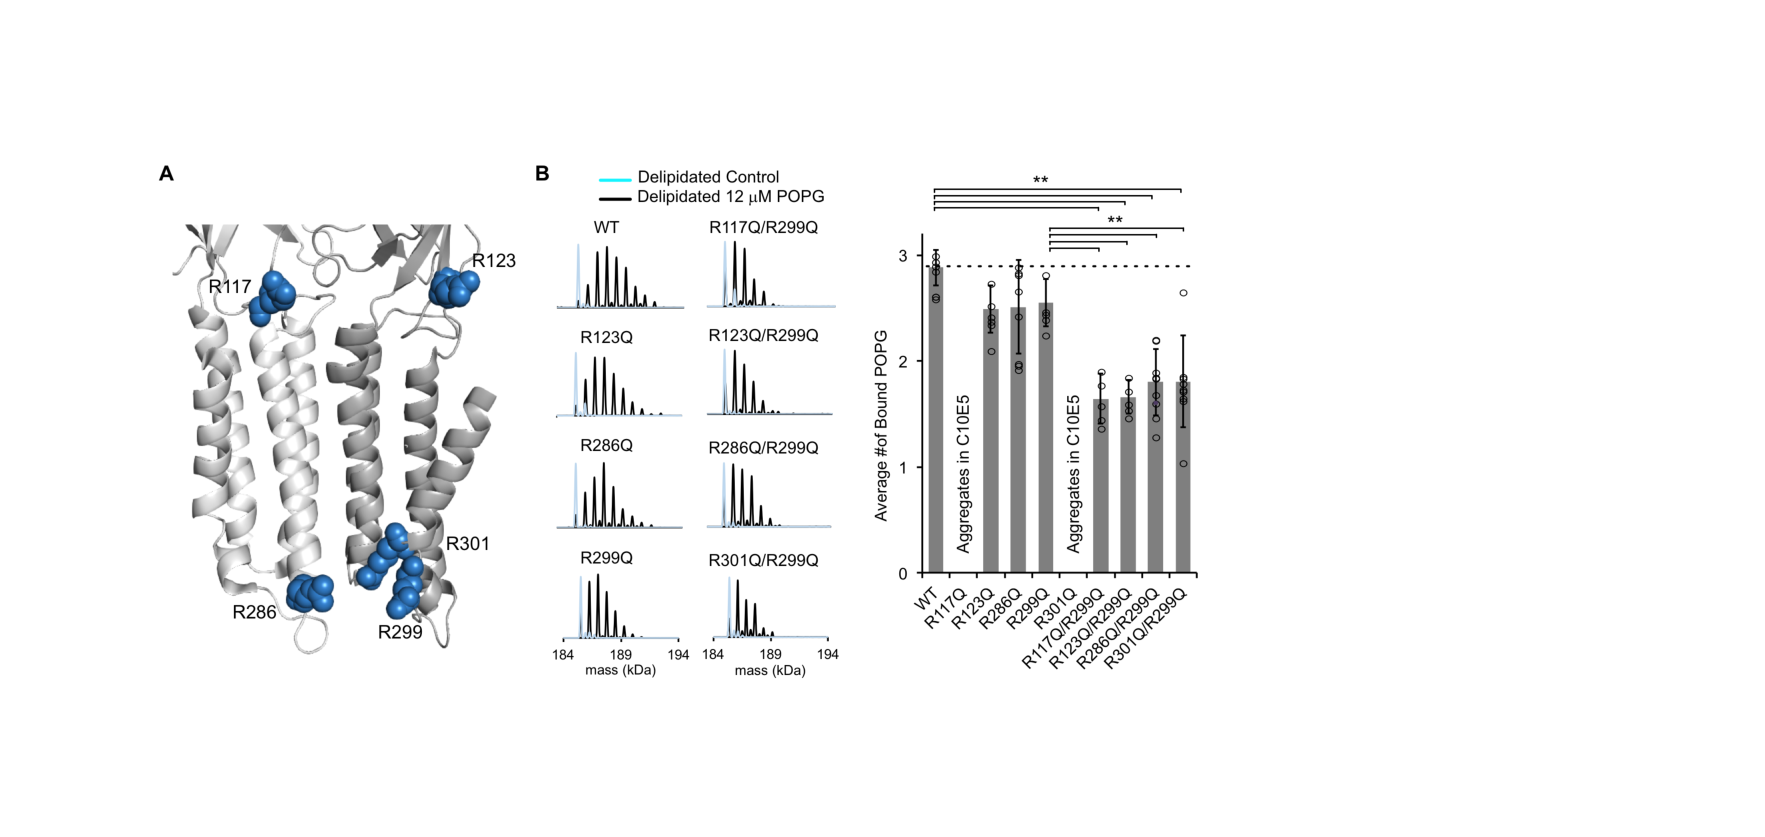
\includegraphics[width=1\linewidth]{./pandoc_test/media/image5.pdf}
\caption[Mutations of five interfacial arginines reduce POPG binding.] {Mutations of five interfacial arginines reduce POPG binding.(A) Structure of ELIC showing two adjacent subunits and five arginine side chains that were mutated to glutamine. (B) Left: Representative deconvoluted spectra of ELIC WT and indicated mutants. Blue indicates spectra of delipidated ELIC in C10E5. Black indicates spectra of delipidated ELIC in C10E5 with 12 $\mu$M POPG. Right: Plot of average number of bound POPG for ELIC WT and mutants, delipidated in C10E5, with 12 $\mu$M POPG (n=5-8, $\pm$SD, **p$<$0.01).} \label{fig:six}
\end{figure*}

In other ion channels, guanidine groups from interfacial arginine side
chains are thought to mediate binding of anionic phospholipids by charge
interactions with the phospholipid headgroup (9, 38). To test the
hypothesis that this mechanism is present in a pLGIC, we mutated all
five arginines in the inner and outer interfacial regions of the ELIC
TMD to glutamine (Fig. \ref{fig:six}A). Phospholipid binding was then assessed by
delipidating each mutant in C10E5, and measuring binding of POPG by
native MS. While R123Q, R286Q, and R299Q could be stably delipidated,
R117Q and R301Q aggregated (Fig. \ref{fig:six}B). However, we found that double
mutants with R299Q (i.e. R117Q/R299Q and R301Q/R299Q) could be stably delipidated. Thus, double
mutants of all arginine mutants in combination with R299Q were expressed
and delipidated (Fig. \ref{fig:six}B). In the presence of 12 $\mu$M POPG, the single
mutants showed moderate decreases (13-18\%) in the average number of
bound POPG compared to WT (Fig. \ref{fig:six}B). This decrease was not statistically
significant. However, all double mutants significantly decreased the
average number of bound POPG relative to WT by 38-41\% and relative to
R299Q by 27-32\% (Fig. \ref{fig:six}B). These results indicate that each interfacial
arginine contributes approximately equally to POPG binding in ELIC. It
is likely that significant decreases in binding could only be
appreciated in the double mutants because of the variability in the
data.

\begin{figure*}
\center
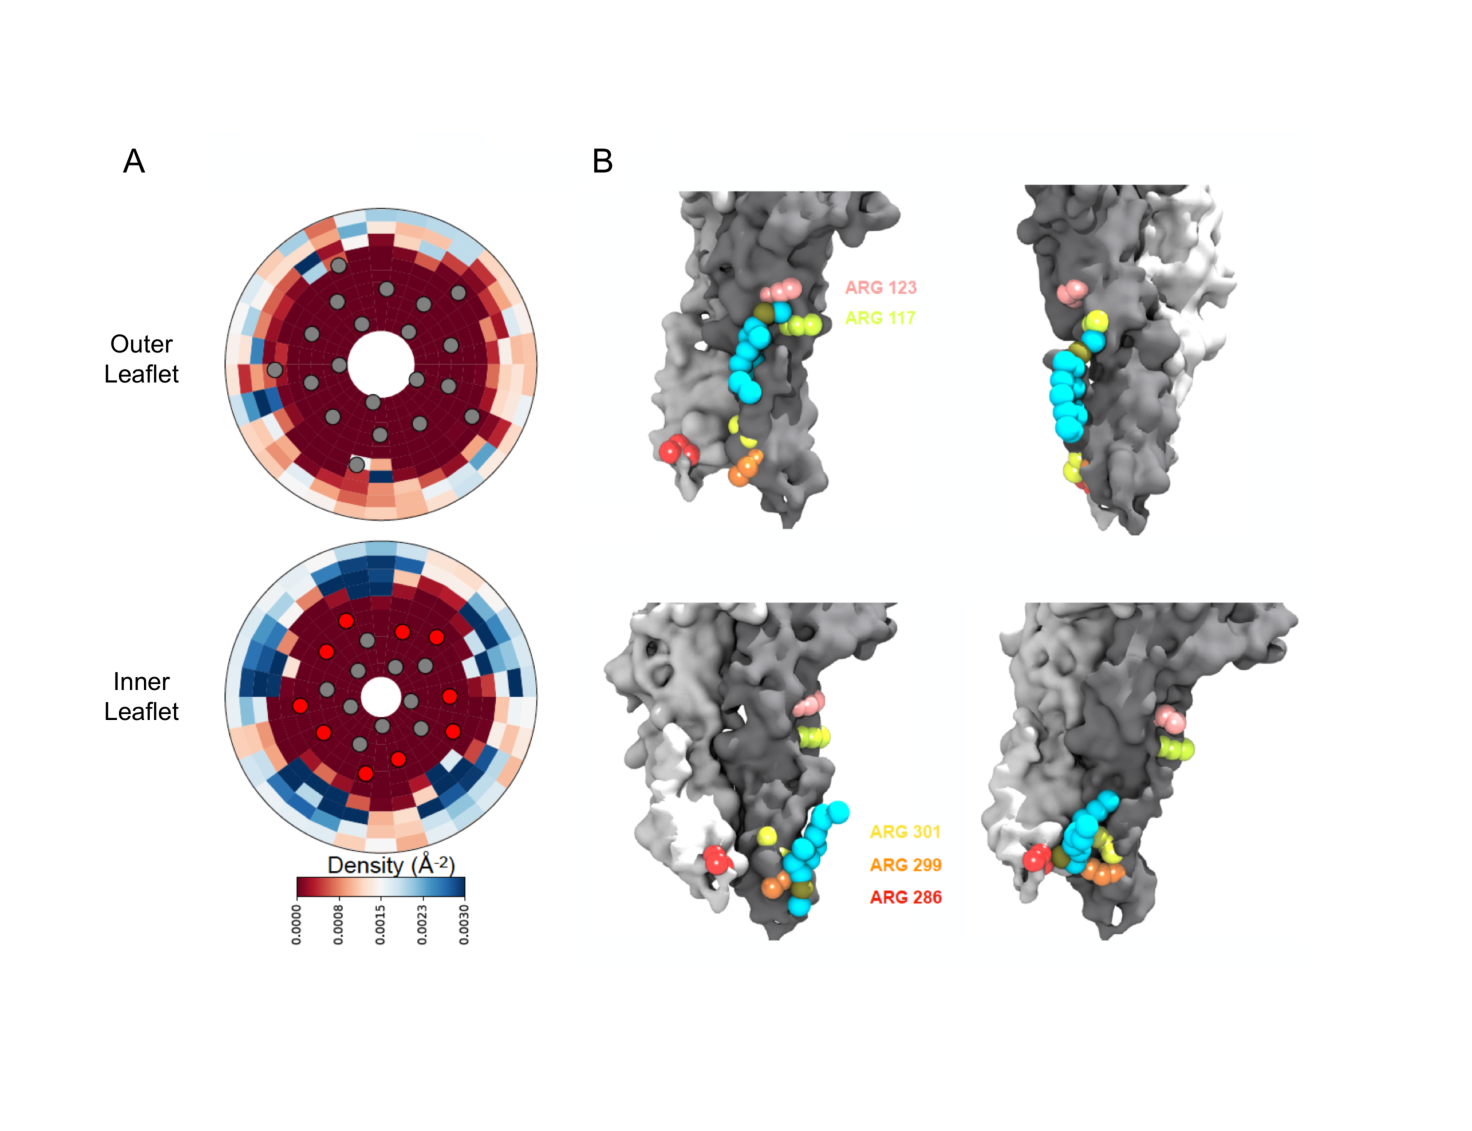
\includegraphics[width=\linewidth]{./pandoc_test/media/image6.pdf}
	\begin{flushleft}

\caption[Density calculations of lipids in binary membranes and visualization of direct POPG-ELIC interactions at 10\% POPG.] {Density calculations of lipids in binary membranes and visualization of direct POPG-ELIC interactions at 10\% POPG. (A) Distribution of POPG density in a POPG-POPC membrane, within 40 $\AA$ from the ELIC pore over the last half of a 15 $\mu$s simulation, for both the outer leaflet (top) and the inner leaflet (bottom). Density is colored according to the color bar, where red and blue represent low and high POPG density, respectively. Circles represent the ELIC transmembrane backbone center of mass, with the helices containing the interfacial arginines colored in red (B) Representative frames after ~9 $\mu$s of simulation, showing multiple POPG binding modes associated with high density areas in (A). Two adjacent subunits of ELIC are shown in grey and white, while arginine side chains of interest are colored in peach, lime-yellow, orange, yellow, and red. POPG phosphate is colored in tan with the rest of the lipid in cyan.} \label{fig:seven}
	\end{flushleft}

\end{figure*}



We further examined these sites of interaction using our coarse-grained
MD simulations. To identify whether boundary POPG were localized around
specific helices or residues, two-dimensional densities of the
negatively-charged headgroup bead were calculated. The distributions are
separated by leaflet where each leaflet contained 10\% POPG. As shown in
Fig. \ref{fig:seven}A, POPG was more likely to interact with ELIC in the inner
leaflet than the outer leaflet, consistent with three out of five
interfacial arginines residues being located on the intracellular
interface of the ELIC TMD. These three arginines are located on TM3
(R286) and TM4 (R299 and R301). Contacts between POPG and all three of
these residues are also visible in individual frames of the simulation
(Fig. \ref{fig:seven}B). Moreover, POPG is more likely to be contacting the
interfacial residues in TM4 (such as R299 and R301) than accessible
interfacial residues in any other helices (Fig. \ref{fig:seven}A). The remaining two
arginine residues are located at the TMD-ECD interface (R117 and R123).
POPG density in the outer leaflet localized to these residues at
intrasubunit sites between TM4 and TM1 or TM4 and TM3 (Fig. \ref{fig:seven}A), and
contacts between these residues and POPG headgroups in the outer leaflet
were also observed in snapshots from the MD simulations (Fig. \ref{fig:seven}B). In
summary, the native MS data and coarse-grained MD simulations
demonstrate that five interfacial arginines contribute to specific POPG
binding sites in the inner and outer leaflets adjacent to TM4.

\subsection{Specific interfacial arginines mediate POPG effect}

Having established that ELIC selectively binds POPG over neutral
phospholipids, and that binding is mediated by five interfacial
arginines, we examined the role of these binding sites on ELIC
desensitization. We reconstituted each single mutant into giant
liposomes composed of a 2:1:1 ratio of POPC:POPE:POPG (25\% POPG) to
test channel function by excised patch-clamping. We hypothesized that
since increasing mole\% POPG decreases ELIC desensitization, certain
arginine mutants, which disrupt POPG binding, may increase ELIC
desensitization. Indeed, all five single arginine mutants showed
variable increases in the rate or extent of desensitization; however,
these differences were generally small and statistically insignificant
except for R301Q (Fig. \ref{fig:eight}, Fig. \ref{fig:nine}). We also tested the double mutants,
which showed significant decreases in POPG binding. Three double mutants
(R117Q/R299Q, R123Q/R299Q, R301Q/R299Q) showed a significant increase in
the extent of desensitization while two (R117Q/R299Q, R301Q/R299Q) also
showed a significant increase in the rate of desensitization (Fig. \ref{fig:eight},
Fig. \ref{fig:nine}). The effects observed in the double mutants approximate the sum
of effects observed in the single mutants. Only R286Q/R299Q did not
affect the extent or rate of desensitization (Fig. \ref{fig:eight}, Fig. \ref{fig:nine}). The
EC\textsubscript{50} of cysteamine response and activation kinetics were
also measured for all mutants; only R117Q and R117Q/R299Q showed
significantly lower EC\textsubscript{50} and activation tau values
compared to WT (Fig. \ref{fig:nine}, Fig. \ref{fig:Supplementary Fig. 7}). Overall, these data
indicate that four of five interfacial arginine residues that reduce
POPG binding (i.e. R117, R123, R299, R301) also increase the rate and/or
extent of ELIC desensitization.

\subsection{L240A reduces desensitization and enhances POPG binding}

If mutations that disrupt POPG binding increase receptor
desensitization, then a mutation that decreases desensitization may
enhance POPG binding. Mutation of a conserved pore-facing 9' TM2 leucine
residue is known to slow desensitization in ELIC (L240A) (36) and other
pLGICs. To confirm this finding in our system, we reconstituted ELIC
L240A into giant liposomes for patch-clamping and observed a significant
reduction in the extent and rate of desensitization (Fig. \ref{fig:ten}A). To
examine POPG binding, L240A was then de-lipidated in C10E5 for native
MS. Interestingly, L240A significantly increased POPG binding compared
to WT at 12 $\mu$M POPG (\textasciitilde{}1.7x increase in average number of
POPG bound) (Fig. \ref{fig:ten}B).


\begin{figure*}

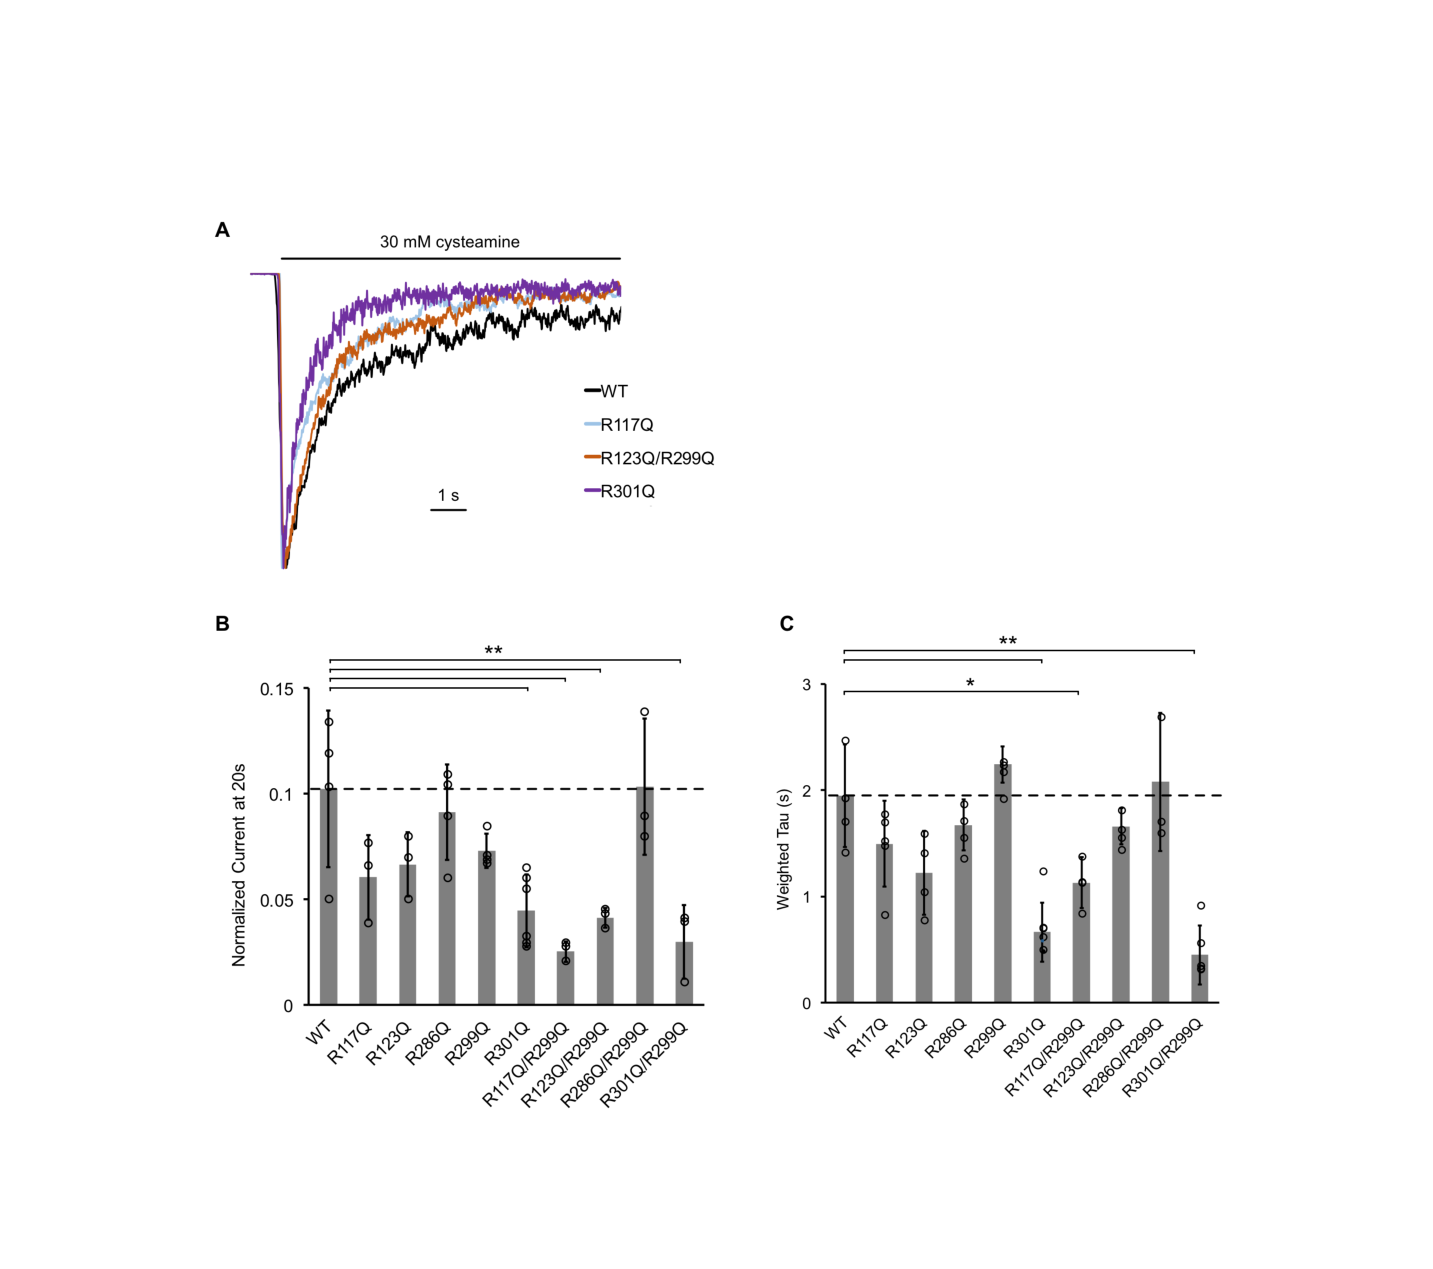
\includegraphics[width=\linewidth]{./pandoc_test/media/image7.pdf}

\caption[The effect of ELIC mutants on desensitization.] {The effect of ELIC mutants on desensitization. (A) Normalized ELIC WT and mutant current responses to 30 mM cysteamine in 25\% POPG liposomes. (B) Graph of ELIC WT and mutant currents 20 s after application of 30 mM cysteamine normalized to peak response in 25 mole\% POPG liposomes (n=3-7, $\pm$SD, **p$<$0.01, *p$<$0.05). (C) Same as (B) for weighted tau (time constants) of desensitization.} 
\label{fig:eight}

\end{figure*}

\section{Discussion}

Recent structural and computational evidence suggests that lipids bind
to pLGICs at specific sites within the TMD (24, 25, 39-41). However,
there is a scarcity of evidence showing that changes in direct lipid
binding are correlated with functional effects (25). We show that the
anionic phospholipid, POPG, selectively binds to ELIC using native MS,
thermally stabilizes the channel, and decreases receptor
desensitization. Overall, these data support the idea that lipid binding
directly affects receptor stability and function. Further, mutations of
arginine residues that reduce POPG binding also increase ELIC
desensitization to varying degrees. While it is possible that these
arginine mutations increase desensitization through a mechanism other
than their effect on POPG binding, the correlation between binding and
desensitization, and the finding that the L240A mutation, which reduces
desensitization, increases POPG binding affinity supports this
conclusion. Remarkably, the L240A mutation, which is located in the
channel pore and remote from the lipid interface (Fig. \ref{fig:eleven}), appears to
allosterically alter the affinity of ELIC for POPG. It is expected that
a mutation that stabilizes a higher affinity state of the receptor (e.g.
active over desensitized) would also enhance binding. Lipids may
modulate ion channel activity through indirect effects on the physical
properties of the membrane or through direct binding interactions (42,
43). The lipid binding data presented in this study using native MS
provides evidence that direct binding of anionic phospholipids
allosterically stabilizes the open state of a pLGIC relative to the
desensitized state.

\begin{figure*}

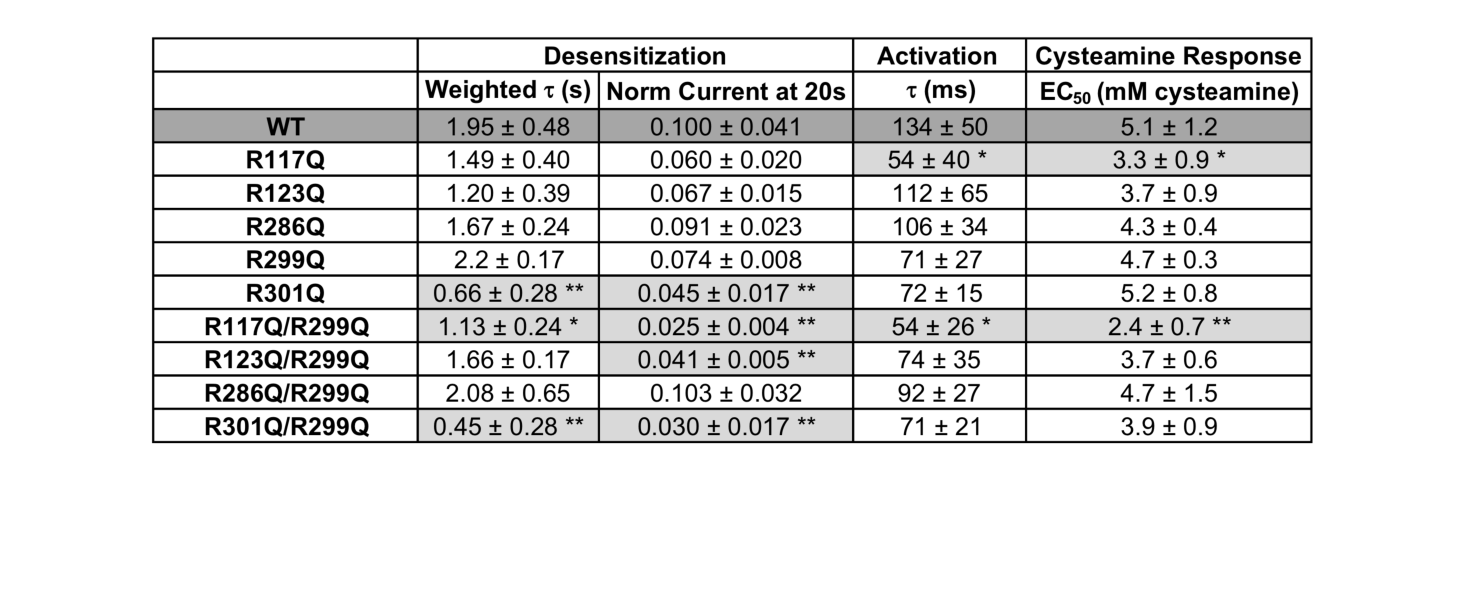
\includegraphics[width=\linewidth]{./pandoc_test/media/image8.pdf}

\caption[ELIC WT and mutant channel properties in giant liposomes composed of 25 mole\% POPG (n=3-7, $\pm$SD).] {ELIC WT and mutant channel properties in giant liposomes composed of 25 mole\% POPG (n=3-7, $\pm$SD). Shown are weighted time constants ($\tau$) for desensitization and currents 20 s after application of 30 mM cysteamine normalized to peak response. Also shown are activation time constants and EC50 of cysteamine response. Light gray indicates mutant values which are significantly different from WT (dark gray) (** p$<$0.01, * p$<$0.05).} 
\label{fig:nine}

\end{figure*}

Membrane proteins including pLGICs are thought to determine their lipid
microenvironment by specific binding interactions (28, 44). Our native
MS measurements provide unique insights into phospholipid interaction
with a pLGIC. First, we find that more POPG binds to ELIC compared to
POPE or POPC at equivalent concentrations, suggesting that POPG binds to
ELIC with higher affinity. This is supported by enrichment of POPG
compared to POPE in phospholipids that are co-purified with ELIC, and
coarse-grained simulations which show enrichment of POPG among the
boundary phospholipids of ELIC. Second, native MS also allows
determination of the stoichiometry and sites of lipid binding (32, 45).
By relating binding stoichiometry and thermal stability, the data
estimate that 32 POPG lipids, which is the average predicted number of
annular lipids in ELIC from MD simulations, results in greater than 80\%
of the stabilizing effect against thermal denaturation (Fig. \ref{fig:Supplementary
Fig. 5}), suggesting that maximal thermal stability is achieved when the
entire ELIC transmembrane domain (TMD) is surrounded by POPG. Although
five interfacial arginine residues were identified to contribute to POPG
binding in ELIC (25 arginines total), it is conceivable that each
arginine side chain may interact with more than one phospholipid
headgroup or that other sites exist.

To quantify the effect of the ELIC double mutants on specific POPG
binding sites, we also fit the native MS binding data for the double
mutants to a binomial binding model using the dissociation constant for
POPG binding to WT and varying the number of available sites. POPG
binding to the double mutants was best fit with a reduction in the
number of available sites from 32 in WT to 18-21 in the mutants
(Fig. \ref{fig:Supplementary Fig. 4}). Given the \textasciitilde{}35-45\% decrease in
bound phospholipid with each double mutant (mutation of two out of five
arginines), we conclude that phospholipid binding at these residues
constitute the highest affinity sites. This is indeed consistent with
the POPG densities from the coarse-grained simulations, which show
discrete enrichment of POPG lipids adjacent these residues. Disruption
of binding sites by mutation of these arginines may not prevent the
occupancy of lipids at these sites per se, but may alter the lipid
binding modes or occupancy times at these sites.

\begin{figure*}
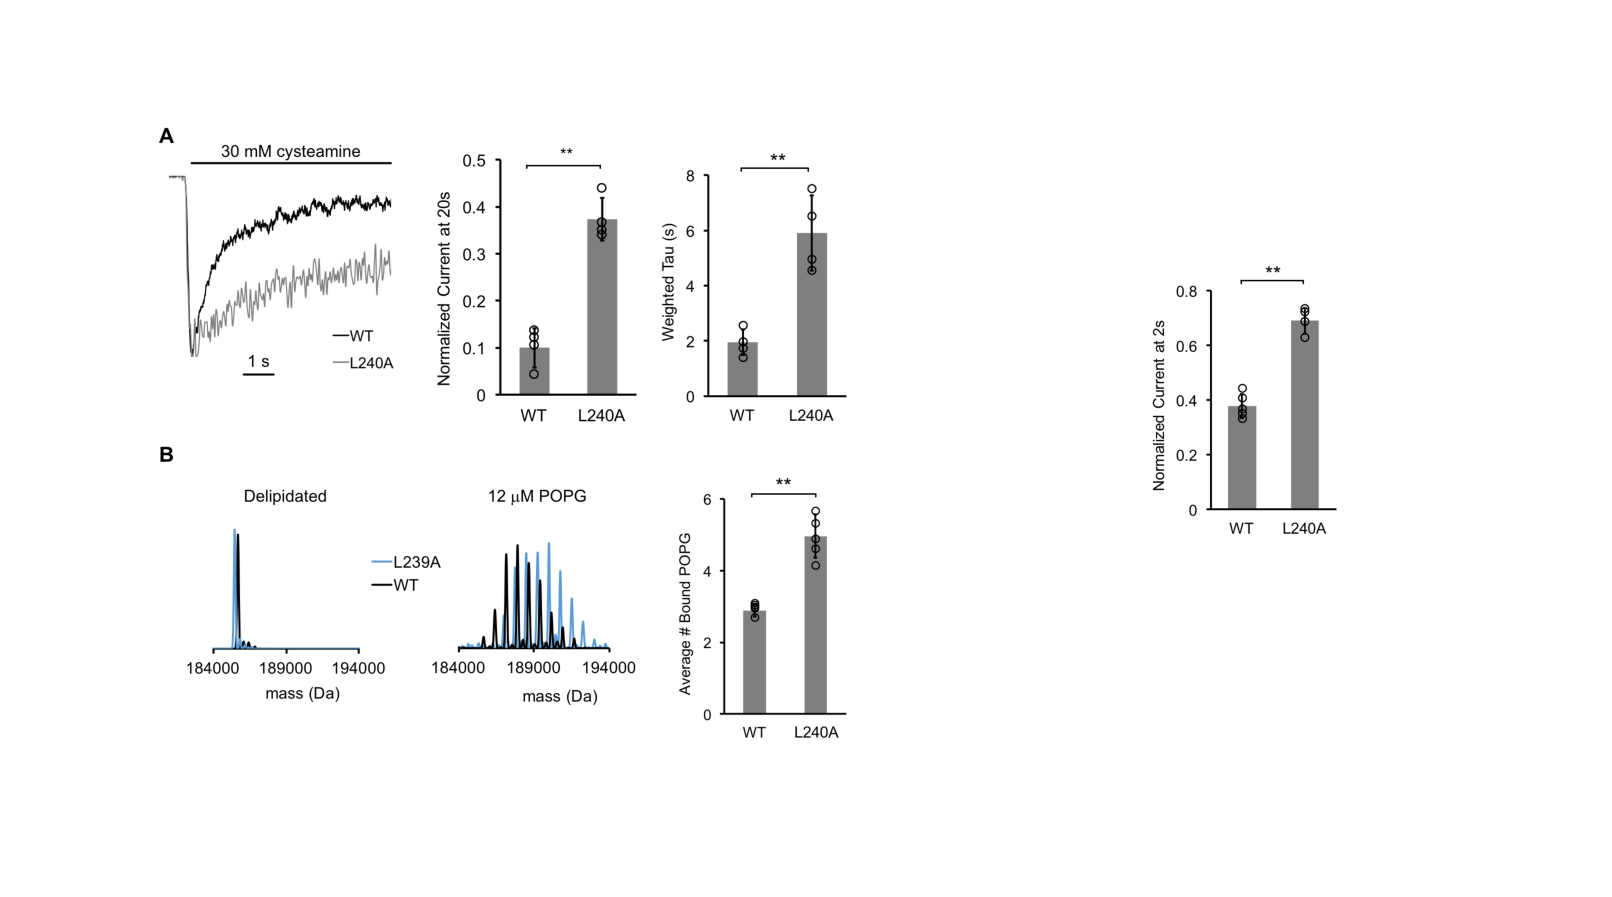
\includegraphics[width=\linewidth]{./pandoc_test/media/image9.pdf}
\caption[The L240A mutant decreases desensitization and increases POPG binding.] {The L240A mutant decreases desensitization and increases POPG binding. (A) Left: Normalized ELIC WT and L240A current responses to 30 mM cysteamine in 25\% POPG liposomes. Middle: ELIC WT and L240A currents 20 s after application of 30 mM cysteamine normalized to peak response at 25 mole\% POPG (n=4-5, $\pm$SD, **p$<$0.01). Right: Weighted tau (time constants) of ELIC WT and L240A desensitization time courses at 25 mole\% POPG (n=4-5, $\pm$SD, **p$<$0.01). (B) Left: Representative deconvoluted spectra of ELIC WT (black) and L240A (blue) showing ELIC delipidated in C10E5 without and with 12 $\mu$M POPG. Right: Graph of average number of bound POPG for ELIC WT and L240A, delipidated in C10E5, with 12 $\mu$M POPG (n=4-5, $\pm$SD, **p$<$0.01).}  \label{fig:ten}
\end{figure*}

Previous studies examining the effects of lipids on pLGIC function found
that nAchR and ELIC are inactive in POPC-only membranes (6, 15, 30), and
it was proposed that this is due to uncoupling of agonist binding to
channel activation (46). To examine ELIC channel activity in liposomes
lacking anionic phospholipid, we utilized a stopped-flow flux assay, and
demonstrated cysteamine-elicited flux by ELIC in POPC-only liposomes.
The high sensitivity of this assay may be the reason ELIC activity could
be detected, contrary to a prior study in which ELIC in POPC liposomes
were injected into \textit{Xenopus} oocytes (30). However, the ELIC
activity was significantly decreased compared to POPC:POPE:POPG (2:1:1)
liposomes. The low protein concentration used in this assay does not
allow us to assess the reconstitution efficiencies. Thus, the overall
lower flux rates and smaller amplitudes in POPC could stem from lower
protein reconstitution. However, the faster desensitization kinetics in
POPC liposomes can be resolved reliably, and are consistent with the
patch-clamp measurements. The results substantiate the role of POPG in
stabilizing the open state relative to the desensitized state, and
demonstrate the utility of measuring pLGIC activity in liposomes of
defined lipid composition using complementary
patch-clamp
and stopped-flow flux techniques.

\begin{figure*}
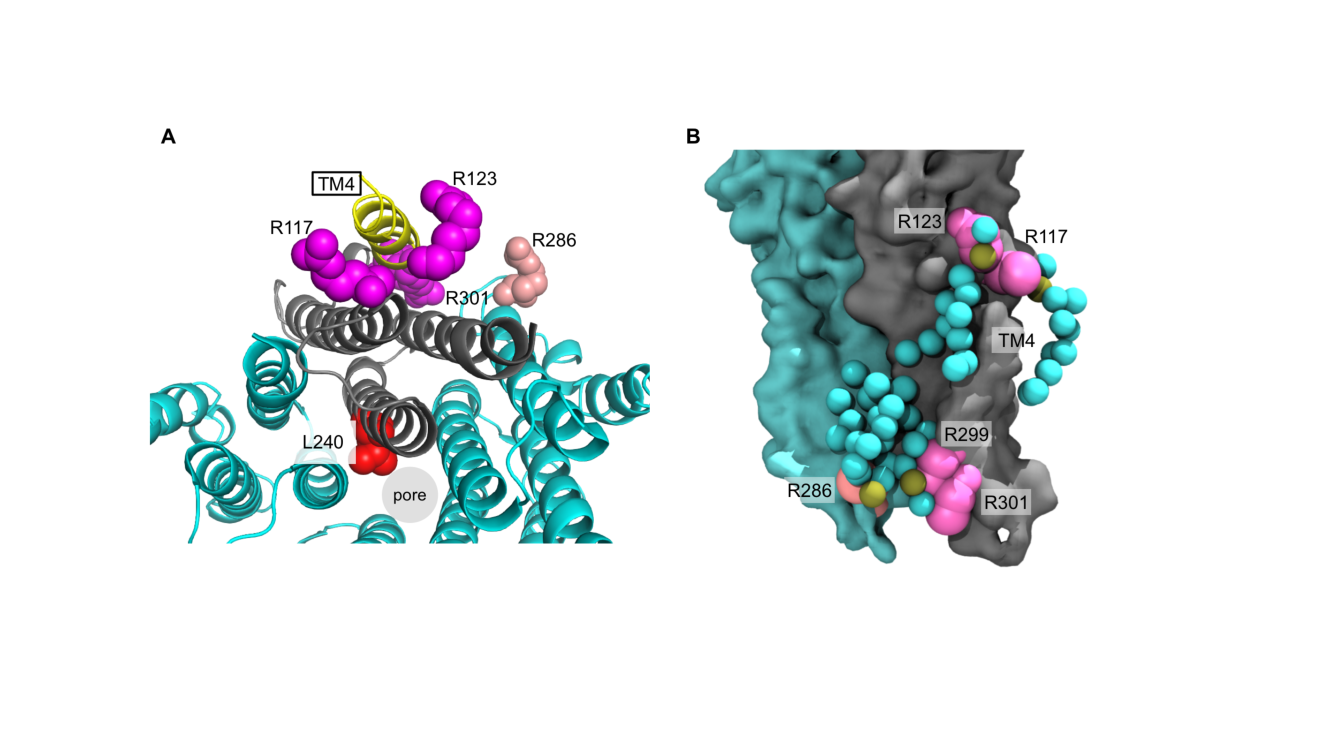
\includegraphics[width=\linewidth]{./pandoc_test/media/image10.pdf}
\caption[Arginines involved in POPG binding and ELIC desensitization.] {Arginines involved in POPG binding and ELIC desensitization. (A) Top view of ELIC highlighting TM4 (yellow) and showing the side chains of R117, R123 and R301 (magenta) adjacent to TM4, which increase ELIC desensitization, and R286 at the subunit interface (salmon), which has no effect on desensitization. L240 (red) faces the pore. (B) Image from coarse-grained simulations with 50\% POPG showing two adjacent ELIC subunits and the mutated arginine side chains (R117, R123, R299 and R301 in magenta; R286 in salmon). Also, shown are all POPG lipids making contacts with the TMD in this snapshot.} \label{fig:eleven}
\end{figure*}

While pLGICs are known to be sensitive to their lipid environment, the
binding sites that mediate lipid modulation are not well defined. It has
been proposed that TM4 is a lipid sensing structure in pLGICs due to its
proximity to the lipid membrane and sensitivity to mutagenesis (41,
47-49). Furthermore, crystal structures of GLIC show bound lipids within
intrasubunit grooves between TM4-TM1 and TM4-TM3 (23), which have been
proposed to be important determinants of channel opening (24, 25).
Photolabeling studies have also identified intrasubunit neurosteroid
binding sites adjacent to TM4 that mediate neurosteroid modulatory
effects (50, 51). We show that POPG binding at multiple interfacial
arginine residues, including R117, R124, R299 and R301 which are
localized to the extracellular and intracellular sides of TM4 (Fig. \ref{fig:eleven}),
are likely important in mediating the effect of POPG on ELIC
desensitization. Examination of boundary POPG from coarse-grained
simulations with high POPG mole\% (50\%) at 15 $\mu$s shows POPG headgroups
making contacts with all of these arginine side chains, and illustrates
potential binding modes for the acyl chains (Fig. \ref{fig:eleven}B). For example,
boundary POPG with headgroups that interact with R301 or R299 have acyl
chains that make contacts with intrasubunit sites along the
intracellular side of TM4 (Fig. \ref{fig:eleven}B and 5B). R301, which has the largest
effect on desensitization when mutated, is conserved among many
mammalian pLGICs including GABA\textsubscript{A}R and nAchR isoforms,
and R299 is adjacent to R301 at the bottom of TM4. Mutations in this
region of TM4 have profound effects on pLGIC desensitization (48, 49,
52, 53). R117 and R123 are located at the extracellular end of TM4, and
boundary POPG with headgroups that interact with these residues have
acyl chains that make contacts with intrasubunit sites on both sides of
TM4 (Fig. \ref{fig:eleven}B and 5B). Sites equivalent to R117 and R123 in GLIC were
previously found to be occupied by a phospholipid and docosahexaenoic
acid (DHA), respectively (24, 25). The polyunsaturated fatty acid, DHA,
was found to increase desensitization in GLIC (25). Therefore, it is
possible that the exact lipid structure occupying these sites results in
different effects. Our results raise the hypothesis that lipids with
polyunsaturated acyl chains or certain sterols (54) exert the opposite
effect of activating phospholipids by acting as competitive antagonists.

In summary, the anionic phospholipid, POPG, decreases desensitization in
the pLGIC, ELIC. POPG specifically binds to and stabilizes ELIC by
interacting with interfacial arginine residues. Our results strongly
suggest that binding of POPG at specific sites modulates receptor
desensitization.

\section{Methods}

\subsection{Mutagenesis, expression and purification of ELIC}

pET26-MBP-ELIC was a gift from Raimund Dutzler (Addgene plasmid \#
39239) and was used for WT ELIC expression and generation of mutants.
Site-directed mutagenesis was performed by the standard Quikchange
approach, and confirmed by Sanger sequencing (Genewiz, Plainfield, NJ).
WT and mutant ELIC was expressed as previously described (25, 55) in
OverExpressTM C43 (D3) \emph{E. coli} (Lucigen, Middleton, WI). Cultures
were grown in Terrific Broth (Sigma, St. Louis, MO) and induced with 0.1
mM IPTG for \textasciitilde{}16 hours at 18 \textsuperscript{o}C.
Pelleted cells were resuspended in Buffer A (20 mM Tris pH 7.5, 100 mM
NaCl) with cOmplete EDTA-free protease inhibitor (Roche, Indianapolis,
IN), and lysed using an Avestin C5 emulsifier at \textasciitilde{}15,000
psi. Membranes were collected by ultracentrifugation, resuspended in
Buffer A, solubilized in 1 \% DDM (Anatrace, Maumee, OH), and incubated
with amylose resin (New England Biolabs, Ipswich, MA) for 2 hours. The
resin was washed with 20 bed volumes of Buffer A, 0.02\% DDM, 0.5 mM
tris(2-carboxyethyl)phosphine (TCEP) and 1 mM EDTA, and eluted with
Buffer A, 0.02\% DDM, 0.05 mM TCEP, and 40 mM maltose. Eluted protein
was digested overnight with HRV-3C protease (Thermo Fisher, Waltham, MA)
(10 units per mg ELIC) at 4 \textsuperscript{o}C, and injected on a
Sephadex 200 10/300 (GE Healthcare Life Sciences, Pittsburgh, PA) size
exclusion column in Buffer A, 0.02\% DDM.

\subsection{Native MS measurements}

Native MS analysis was similar to previous descriptions for other
membrane proteins (27). For analysis of ELIC in DDM, 30 $\mu$l of purified
protein in 0.02\% DDM at \textasciitilde{}1 mg/ml was buffer exchanged
into 200 mM ammonium acetate pH 7.5 and 0.02\% DDM using Biospin 6 gel
filtration spin columns (Bio-Rad, Hercules, CA). 2 $\mu$l of buffer
exchanged ELIC was loaded into a borosilicate capillary emitter (Thermo
Scientific, Waltham, MA), and analyzed by static nanospray on a Thermo
QExactive EMR mass spectrometer. The following parameters were used to
resolve the ELIC pentamer and minimize dissociation into tetramer and
monomer: capillary voltage of 1.2 kV, capillary temperature of 200
\textsuperscript{o}C, ion transfer optics set with the injection
flatapole, inter-flatapole lens, bent flatapole, transfer multiple as 8,
7, 6, 4 V, respectively, resolution 8,750, AGC target 3 x
10\textsuperscript{6}, trap pressure set to maximum, CID 200 V, and CE
100 V. For analysis of ELIC in C10E5, ELIC delipidated by injecting 300
$\mu$g onto a Sephadex 200 10/300 column (GE Healthcare) at 0.5 ml/min
pre-equilibrated with Buffer A, 10\% glycerol, and 0.06\% C10E5
(Anatrace). 30 $\mu$l aliquots were then buffer exchanged to 100 mM ammonium
acetate pH 7.5, 0.06\% C10E5 using Biospin 6 columns, and diluted to 0.2
mg/ml. MS measurements on the QExactive EMR were performed with the
parameters listed above except: capillary temperature 100
\textsuperscript{o}C, CID 75 V and CE 200 V. For lipid binding
measurements, stocks of POPG lipid were prepared at 2x the concentration
of POPG being tested in 100 mM ammonium acetate pH 7.5 and 0.06\% C10E5.
Lipid stocks were then mixed with 0.4 mg/ml ELIC in a 1:1 volume ratio
for a final concentration of 1 $\mu$M ELIC, and samples were analyzed after
\textgreater{}5 min incubation.

MS spectra were deconvoluted using UniDec (56); deconvolution of spectra
with bound lipid was restricted to the +26 to +22 charge states
(Fig. \ref{fig:Supplementary Fig. 3}). Peak heights of apo and lipid-bound species were
extracted from UniDec, and analyzed by two approaches. The average
number of bound lipids was determined by the following relationship:
\begin{equation}
\mathrm{Average\ number\ bound\ lipid = \ }\frac{\sum_{\mathrm{n = 0}}^{\mathrm{k}}{\mathrm{n \cdot}\mathrm{I}_{\mathrm{n}}}}{\sum_{\mathrm{n = 0}}^{\mathrm{k}}\mathrm{I}_{\mathrm{n}}}
\end{equation}
where n is the number of bound lipids and I\textsubscript{n} is the
deconvoluted peak height of ELIC with n bound lipids. Peak heights of
apo and lipid-bound species were also plotted as mole fraction versus
the number of bound lipids (Fig. \ref{fig:Supplementary Fig. 4}). These data were fit
with a binomial binding model, which assumes that there are N sites each
with equal affinity, K. The probability, p, that a site is occupied at
the concentration of a given lipid, A, is defined as:

\begin{equation}
p = \frac{\lbrack A\rbrack}{\left\lbrack A \right\rbrack + K}
\end{equation}

Then, the probability (B) that q sites are occupied out of N total sites
is given by the binomial probability function:

\begin{equation}
B\left( q \right) = \ \frac{N!}{q!\left( N - q \right)!}p^{N - q}{(1 - p)}^{q}
\end{equation}

B(q) was used to determine the mole fraction of each lipid-bound species
at a given {[}A{]}, which was used to fit the native MS data in Excel
across all {[}A{]} by setting K constant and varying N or vice versa.

\subsection{Thermal stability assay}

Purified WT ELIC in C10E5 (Buffer A, 0.06\% C10E5) was diluted to 1 $\mu$M
in the absence or presence of various concentrations of phospholipid.
Samples were analyzed without and with heating in the absence or
presence of phospholipid. Analysis of protein thermal stability was
performed by injecting 90 $\mu$l of sample on a size exclusion column
(Sephadex 200 10/300), and measuring the amplitude of the pentamer peak
as previously described (57, 58). Heating was performed for 15 min at 32
\textsuperscript{o}C, which resulted in a \textasciitilde{}85\% decrease
in the pentamer amplitude compared to 4\textsuperscript{o}C. The
stabilizing effect of a phospholipid was quantified as the pentamer
amplitude in the presence of phospholipid (heated) divided by control
(heated).

\subsection{Excised patch-clamp recordings from giant liposomes}

ELIC WT and mutants were reconstituted into giant liposomes as
previously described with some modifications (59). Three liposome
preparations were used in this study: 1) 25\% POPG (consists of 50\%
POPC/ 25\% POPE/ 25\% POPG), 2) 12\% POPG (consists of 60\% POPC/ 28\%
POPE/ 12\% POPG), and 3) 40\% POPG (consists of 35\% POPC/ 25\% POPE/
40\% POPG). These liposome compositions were chosen to vary POPG mole\%
while optimizing lipid mixtures to obtain ideal giant liposomes for
patch-clamping. This was achieved by varying POPG mole\% and POPC mole\%
inversely. Condition \#1 was used for WT and all mutants, and conditions
\#2 and \#3 were used in WT. Liposomes were prepared by drying 15-20 mg
of lipid mixtures in chloroform using N\textsubscript{2} in a round
bottom flask and then overnight in a vacuum dessicator. Dried lipids
were rehydrated at 5 mg/ml in 10 mM MOPS pH 7, and 150 mM NaCl (MOPS
buffer), subjected to ten freeze-thaw cycles ten, and then small
unilamellar liposomes were formed by extrusion using a 400 nm filter
(Avanti Lipids, Alabaster, AL) and bath sonication (30 sec x 5). 5 mg of
liposomes in 1 ml were destabilized by adding DDM to 0.2\% and rotating
for 1 hour at room temperature followed by 0.3-0.5 mg of ELIC WT or
mutants at \textasciitilde{}4-5 mg/ml and incubation for 30 min. To
remove DDM, SM-2 Bio-beads (Bio-Rad) were added in five batches (30, 30,
50, 100, and 100 mg). The first three batches were added each hour along
with 1 ml of MOPS buffer to make a final volume of 4 ml while rotating
at room temperature. After adding the first 100 mg batch, the
proteoliposomes were rotated overnight at 4 \textsuperscript{o}C,
followed by the last 100 mg the next day for 3 hours at room
temperature. Proteoliposomes were harvested by ultracentrifugation at
150,000 x \emph{g} for 1 hour at 4 \textsuperscript{o}C, and the pellet
resuspended with 80 $\mu$l of MOPS buffer for a lipid concentration of
\textasciitilde{}50 mg/ml. Giant liposomes were formed by drying 10 $\mu$l
of proteoliposomes on a glass coverslip in a desiccator for 3-5 hours at
4 \textsuperscript{o}C followed by rehydration with 60 $\mu$l of MOPS buffer
overnight at 4 \textsuperscript{o}C and at least 2 hours at room
temperature the next day. Giant liposomes were resuspended by pipetting
and then applied to a petri dish with MOPS buffer.

Patch-clamp recordings were performed using borosilicate glass pipettes
pulled to $\sim2-3$ M$\Omega$ using a P-2000 puller (Sutter
instruments, Novato, CA). Pipettes were filled with 10 mM MOPS pH 7, 150
mM NaCl, and 0.5 mM BaCl$_{2}$. Excised patches (the
orientation of ELIC in the liposomes is not known; therefore, these
patches are not defined as outside-out or inside-out) were held at -60
mV, and bath solutions consisted of 10 mM MOPS pH 7, 150 mM NaCl, 0.5 mM
BaCl$_{2}$, 1 mM DTT, and varying concentrations of
cysteamine. DTT was added to the bath solution to prevent cysteamine
oxidation. Rapid solution exchange was achieved with a three-barreled
flowpipe mounted and adjusted by to a SF-77B fast perfusion system
(Warner Instrument Corporation, Hamden, CT). Liquid junction current at
the open pipette tip demonstrated 10-90\% exchange times of
\textless{}10 ms. Data was collected at 20 kHz using an Axopatch 200B
amplifier (Molecular Devices, San Jose, CA) and a Digidata 1322A
(Molecular Devices) with Axopatch software, and a low pass Bessel filter
of 10 kHz was applied to the currents. Analysis of currents was
performed with Clampfit 10.4.2 (Molecular Devices). Activation currents
were fit to a single exponential equation, and desensitization currents
were fit to both single and double exponential equations. The majority
of desensitization currents were best fit with a double exponential, and
weighted time constants were derived using the following calculation:

\begin{equation}
Weighted \tau = \frac{\left( A1 \cdot \tau 1 \right) + (A2 \cdot \tau 2)}{A1 + A2}
\end{equation}

where A1 and A2 are the weighted coefficients of the first and second
exponential components. The reported weighted average time constants are
averages of weighted time constants from double exponential fits and
time constants from single exponential fits. Peak cysteamine dose
response curves were fit to a Hill equation, keeping n constant at 2,
which provided a reasonable fit for all data sets. All statistical
comparisons were made using a one-way ANOVA with post-hoc Tukey HSD
test.

\subsection{Stopped-flow fluorescence recordings}

The fluorescence-based sequential-mixing stopped-flow assay was carried
out with an SX20 stopped-flow spectrofluorimeter (Applied Photophysics,
Leatherhead, UK) at 25 \textsuperscript{o}C. To reconstitute ELIC into
large unilamellar vesicles (LUVs), 15 mg of lipids (POPC or
POPC:POPE:POPG 2:1:1) were dried in glass vials to a thin film under a
constant N\textsubscript{2} stream. Lipids were further dried under
vacuum overnight. The next day, lipids were rehydrated in reconstitution
buffer (1114 $\mu$l of 15 mM Hepes, 150 mM NaNO\textsubscript{3}, pH 7). 33
mg CHAPS were added stepwise while sonicating lipids in a bath sonicator
until the solution was clear. 1057 $\mu$l of a 75 mM ANTS stock solution (in
ddH\textsubscript{2}O, pH 7) was added together with purified ELIC (1
$\mu$g/mg lipid), mixed and incubated for 20 min. Detergent removal was
initiated by addition of 0.7 g SM-2 BioBeads (BioRad) in assay buffer
(10 mM Hepes, 140 mM NaNO\textsubscript{3}, pH 7). The reconstitution
mix was incubated for 2.5 h at 21 \textsuperscript{o}C under gentle
agitation. The liposome-containing supernatant was transferred to a new
glass tube and stored overnight at 13 \textsuperscript{o}C. The liposome
solution was sonicated in a bath sonicator for 30 s and extruded through
a 0.1 $\mu$m membrane (Whatman) using a mini-extruder (Avanti Polar lipids).
Extra-vesicular ANTS were removed with a 10 ml desalting column (PD-10,
GE Lifesciences). Right before the assay, liposomes were diluted 5-fold
in assay buffer to ensure a good signal to noise ratio.

For the assay, ELIC-containing liposomes were mixed 1:1 with pre-mix
buffer (assay buffer supplemented with 10 mM cysteamine to reach 5 mM
after mixing) and incubated for defined amounts of time (10 ms -- 25 s).
A second 1:1 mixing step was performed with quenching buffer (10 mM
Hepes, 90 mM NaNO\textsubscript{3}, 50 mM TlNO\textsubscript{3}, pH 7).
ANTS fluorescence was excited at 360 nm and the integral fluorescence
above 420 nm was recorded for 1 s. For each delay time, at least 8
repeats under identical conditions were performed.

To analyze the data, each repeat was visually inspected and outliers
were removed. Each remaining repeat was then fitted to a stretched
exponential (Equation 4.1) and the rate of Tl+ influx was determined at 2
ms (Equation 4.2).
\begin{equation}
F_{t} = F_{\infty}\  + \ \left( F_{0}\  - \ F_{\infty} \right)\  \cdot \ e^{\left\{ - \ \left( \frac{t}{\tau} \right)^{\beta} \right\}}
\end{equation}
\begin{equation}
k_{t} = \ \left( \frac{\beta}{\tau} \right)\  \cdot \ \left( \frac{2\ ms}{\tau} \right)^{\left( \beta\  - 1 \right)}\ 
\end{equation}
with F\textsubscript{t}, F\textsubscript{$\infty$}, F\textsubscript{0} being
the fluorescence at time t, the final fluorescence and the initial
fluorescence, respectively. t is the time (in s), $\tau$ the time constant
(in s) and \emph{$\beta$} the stretched exponential factor.
\emph{k}\textsubscript{t} is the calculated rate (in
s\textsuperscript{-1}) of Thallium influx at 2 ms.

The rate constants were averaged and the mean and standard deviations
(S.D.) were determined and plotted (Fig 2F). The experiments were
repeated for each lipid composition using three independent
reconstitutions. The rates and S.D. were averaged and plotted as
function of the delay time. The time course was fitted according to a
double-exponential function to obtain the rates of activation and
desensitization, respectively.

\subsection{Lipid extraction and MS analysis}

Lipids were extracted using a Bligh-Dyer extraction (60). Briefly, 100
$\mu$g of purified ELIC in DDM and 150 $\mu$g of \emph{E. coli} membranes
derived from cell cultures transformed and induced for ELIC expression,
respectively, were mixed with 1 ml chloroform, 2 ml methanol and 0.8 ml
water, and vortexed for 1 min, followed by an additional 1 ml chloroform
and 1 ml water, and vortex for 3 min. The samples were centrifuged for 3
min at 500 x \emph{g}, and the lower organic phase removed for analysis,
using a Thermo Scientific LTQ Orbitrap Velos mass spectrometer. Lipid
extracts were loop injected (1.5 $\mu$l/min) using a syringe pump that
delivered a continuous flow of methanol at 15 $\mu$l/min into the ESI
source. High resolution (R = 100,000 at m/z 400) MS and MS/MS analyses
were performed in negative ion mode. The skimmer of the ESI source was
set at ground potential, electrospray voltage 4 kV, capillary
temperature 300 \textsuperscript{o}C, AGC target 5 x
10\textsuperscript{4}, and maximum injection time 50 ms.
MS\textsuperscript{n} experiments for identification of lipid structures
were carried out with an optimized relative collision energy of 32\%,
activation q value of 0.25, activation time of 10 ms, and mass selection
window of 1 Da.

\subsection{Coarse-grained simulations of ELIC}

All simulations reported here used the MARTINI 2.2 (61) coarse-grained
topology and force field. The crystal structure of ELIC (PDB 3RQW) (62)
was coarse-grained using MARTINI martinize.py script. Secondary
structural restraints were constructed using martinize.py while imposed
through Gromacs (63). Conformational restraints were preserved through
harmonic bonds between backbone beads less than 0.5 nm apart with a
coefficient of 900 kJ mol\textsuperscript{-1}. Pairs were determined
using the ElNeDyn algorithm (64). Membranes were constructed using the
MARTINI script insane.py (61). The insane.py script randomly places
lipids throughout both inner and outer membranes and embeds selected
proteins into the membrane. Two series of simulations were developed,
the first using POPE and POPG, and the second POPC and POPG. Box sizes
were about 30 x 30 x 25 nm\textsuperscript{3} and each simulation box
contained about 3000 lipids.

Molecular dynamics simulations were carried out using GROMACS 5.1.4
(63). All systems were run using van der Waals (vdW) and electrostatics
in cutoff and reaction-field, respectively, with a dielectric constant
of \(\varepsilon = 15\). vdW and electrostatics used a cutoff length of
1.1 nm as defined in current MARTINI build specifications. Energy
minimizations were performed for about 30,000 steps. All systems were
run for short equilibration steps. Canonical ensembles (NVT) were run
for 100 ps using Berendsen thermostat set to 323 K with the temperature
coupling constant set to 1 ps. Isothermal-Isobaric ensemble (NPT)
equilibration was run for 5000 ps using Berendsen thermostat and
barostat. The thermostat was set to 323 K with the temperature coupling
constant set to 1 ps, and the barostat was set to a pressure coupling
constant of 3 ps with a compressibility of 3 x 10\textsuperscript{-5}
bar\textsuperscript{-1} holding at 1 bar. Molecular dynamics were
carried out using NPT ensemble and were simulated for 15 $\mu$s with a time
step of 0.015 ps using v-rescale thermostat set to 323 K and a
temperature coupling constant of 1 ps. Membranes consisting of POPE used
the Parrinello-Rahman barostat, and membranes consisting of POPC used
the Berendsen barostat, both under semi-isotropic coupling. The
reference pressure was set to 1 bar, the compressibility
3x10\textsuperscript{-4} bar\textsuperscript{-1}, and the pressure
coupling constant 1 ps.

Annular lipids were determined using the annular lipid metric B:
\begin{equation}
B_{i} = \left\langle \frac{b_{i}}{b_{\text{tot}}} \right\rangle\frac{1}{x_{i}} - 1
\end{equation}

where \(b_{i}\) is the instantaneous number of boundary lipids of
species \(i\), \(b_{\text{tot}}\) is the instantaneous total number of
boundary lipids, \(x_{i}\) is the overall (bulk) fraction of species
\(i\) and the brackets represent an average over time and replicas.
\(B_{i}\) \textless{} 0 and \(B_{i}\) \textgreater{} 0 indicate
enrichment and depletion of species \(i\), respectively, relative to the
abundance in the bulk membrane. A given lipid was counted as a boundary
lipid if it was within 6 Å of the ELIC transmembrane domain.

Two dimensional lipid density distributions around a central ELIC
pentamer were calculated for each leaflet using polar coordinates (28).
For every sampled frame, all lipids of species \(i\) were separated into
leaflets. For all \(i\) lipids in a given leaflet, the vector separating
the phosphate beads from ELIC center was calculated and projected onto
the membrane plane. The two-dimensional separation vector was then used
to assign the lipid to the appropriate polar bin of radial bin width
\(4\mathring{\mathrm{A}}\) and angular bin width
\(\frac{\pi}{15}\text{.\ }\)The area density in each bin was averaged
over time and replicas.

\textbf{\emph{\\
}}

\textbf{\emph{Acknowledgements}}

We are grateful to Alex Evers, Joe Henry Steinbach, Christopher Lingle
and Gustav Akk for helpful discussions and edits regarding this study
and the preparation of the manuscript. We also acknowledge Arthur
Laganowsky and Yang Liu for guidance with regard to sample preparation
of ELIC for native MS measurements. We are indebted to Michael Gross at
the Washington University NIH/NIGMS-supported biomedical mass
spectrometry resource for use of the Thermo QExactive EMR mass
spectrometer, and Christopher Lingle for use of a patch-clamp rig for
electrophysiology recordings.

\textbf{\emph{Competing Interests}}

The authors declare that no competing interests exist.

\section{Reference}

1. Corringer PJ, Poitevin F, Prevost MS, Sauguet L, Delarue M, Changeux
JP. Structure and pharmacology of pentameric receptor channels: from
bacteria to brain. Structure. 2012;20(6):941-56.

2. Allen JA, Halverson-Tamboli RA, Rasenick MM. Lipid raft microdomains
and neurotransmitter signalling. Nat Rev Neurosci. 2007;8(2):128-40.

3. Baenziger JE, Henault CM, Therien JP, Sun J. Nicotinic acetylcholine
receptor-lipid interactions: Mechanistic insight and biological
function. Biochim Biophys Acta. 2015;1848(9):1806-17.

4. Rosenhouse-Dantsker A, Mehta D, Levitan I. Regulation of ion channels
by membrane lipids. Compr Physiol. 2012;2(1):31-68.

5. Evers AS, Elliott WJ, Lefkowith JB, Needleman P. Manipulation of rat
brain fatty acid composition alters volatile anesthetic potency. J Clin
Invest. 1986;77(3):1028-33.

6. Criado M, Eibl H, Barrantes FJ. Functional properties of the
acetylcholine receptor incorporated in model lipid membranes.
Differential effects of chain length and head group of phospholipids on
receptor affinity states and receptor-mediated ion translocation. J Biol
Chem. 1984;259(14):9188-98.

7. Cheng WW, D'Avanzo N, Doyle DA, Nichols CG. Dual-mode phospholipid
regulation of human inward rectifying potassium channels. Biophys J.
2011;100(3):620-8.

8. Chemin J, Patel AJ, Duprat F, Lauritzen I, Lazdunski M, Honore E. A
phospholipid sensor controls mechanogating of the K+ channel TREK-1.
EMBO J. 2005;24(1):44-53.

9. Hite RK, Butterwick JA, MacKinnon R. Phosphatidic acid modulation of
Kv channel voltage sensor function. Elife. 2014;3.

10. Schmidt D, Jiang QX, MacKinnon R. Phospholipids and the origin of
cationic gating charges in voltage sensors. Nature.
2006;444(7120):775-9.

11. Zolles G, Klocker N, Wenzel D, Weisser-Thomas J, Fleischmann BK,
Roeper J, et al. Pacemaking by HCN channels requires interaction with
phosphoinositides. Neuron. 2006;52(6):1027-36.

12. daCosta CJ, Medaglia SA, Lavigne N, Wang S, Carswell CL, Baenziger
JE. Anionic lipids allosterically modulate multiple nicotinic
acetylcholine receptor conformational equilibria. J Biol Chem.
2009;284(49):33841-9.

13. Hamouda AK, Sanghvi M, Sauls D, Machu TK, Blanton MP. Assessing the
lipid requirements of the Torpedo californica nicotinic acetylcholine
receptor. Biochemistry. 2006;45(13):4327-37.

14. daCosta CJ, Wagg ID, McKay ME, Baenziger JE. Phosphatidic acid and
phosphatidylserine have distinct structural and functional interactions
with the nicotinic acetylcholine receptor. J Biol Chem.
2004;279(15):14967-74.

15. Ochoa EL, Dalziel AW, McNamee MG. Reconstitution of acetylcholine
receptor function in lipid vesicles of defined composition. Biochim
Biophys Acta. 1983;727(1):151-62.

16. Fong TM, McNamee MG. Correlation between acetylcholine receptor
function and structural properties of membranes. Biochemistry.
1986;25(4):830-40.

17. Baenziger JE, Morris ML, Darsaut TE, Ryan SE. Effect of membrane
lipid composition on the conformational equilibria of the nicotinic
acetylcholine receptor. J Biol Chem. 2000;275(2):777-84.

18. Velisetty P, Chakrapani S. Desensitization mechanism in prokaryotic
ligand-gated ion channel. J Biol Chem. 2012;287(22):18467-77.

19. Ellena JF, Blazing MA, McNamee MG. Lipid-protein interactions in
reconstituted membranes containing acetylcholine receptor. Biochemistry.
1983;22(24):5523-35.

20. Mantipragada SB, Horvath LI, Arias HR, Schwarzmann G, Sandhoff K,
Barrantes FJ, et al. Lipid-protein interactions and effect of local
anesthetics in acetylcholine receptor-rich membranes from Torpedo
marmorata electric organ. Biochemistry. 2003;42(30):9167-75.

21. Dreger M, Krauss M, Herrmann A, Hucho F. Interactions of the
nicotinic acetylcholine receptor transmembrane segments with the lipid
bilayer in native receptor-rich membranes. Biochemistry.
1997;36(4):839-47.

22. Antollini SS, Barrantes FJ. Disclosure of discrete sites for
phospholipid and sterols at the protein-lipid interface in native
acetylcholine receptor-rich membrane. Biochemistry.
1998;37(47):16653-62.

23. Bocquet N, Nury H, Baaden M, Le Poupon C, Changeux JP, Delarue M, et
al. X-ray structure of a pentameric ligand-gated ion channel in an
apparently open conformation. Nature. 2009;457(7225):111-4.

24. Prevost MS, Sauguet L, Nury H, Van Renterghem C, Huon C, Poitevin F,
et al. A locally closed conformation of a bacterial pentameric
proton-gated ion channel. Nat Struct Mol Biol. 2012;19(6):642-9.

25. Basak S, Schmandt N, Gicheru Y, Chakrapani S. Crystal structure and
dynamics of a lipid-induced potential desensitized-state of a pentameric
ligand-gated channel. Elife. 2017;6.

26. Laganowsky A, Reading E, Allison TM, Ulmschneider MB, Degiacomi MT,
Baldwin AJ, et al. Membrane proteins bind lipids selectively to modulate
their structure and function. Nature. 2014;510(7503):172-5.

27. Gault J, Donlan JA, Liko I, Hopper JT, Gupta K, Housden NG, et al.
High-resolution mass spectrometry of small molecules bound to membrane
proteins. Nat Methods. 2016;13(4):333-6.

28. Sharp L, Salari R, Brannigan G. Boundary lipids of the nicotinic
acetylcholine receptor: Spontaneous partitioning via coarse-grained
molecular dynamics simulation. Biochim Biophys Acta Biomembr.
2019;1861(4):887-96.

29. Brannigan G. Direct Interactions of Cholesterol With Pentameric
Ligand-Gated Ion Channels: Testable Hypotheses From Computational
Predictions. Curr Top Membr. 2017;80:163-86.

30. Carswell CL, Sun J, Baenziger JE. Intramembrane aromatic
interactions influence the lipid sensitivities of pentameric
ligand-gated ion channels. J Biol Chem. 2015;290(4):2496-507.

31. Reading E, Liko I, Allison TM, Benesch JL, Laganowsky A, Robinson
CV. The role of the detergent micelle in preserving the structure of
membrane proteins in the gas phase. Angew Chem Int Ed Engl.
2015;54(15):4577-81.

32. Liu Y, LoCaste CE, Liu W, Poltash ML, Russell DH, Laganowsky A.
Selective binding of a toxin and phosphatidylinositides to a mammalian
potassium channel. Nat Commun. 2019;10(1):1352.

33. Nji E, Chatzikyriakidou Y, Landreh M, Drew D. An engineered
thermal-shift screen reveals specific lipid preferences of eukaryotic
and prokaryotic membrane proteins. Nat Commun. 2018;9(1):4253.

34. Zimmermann I, Marabelli A, Bertozzi C, Sivilotti LG, Dutzler R.
Inhibition of the prokaryotic pentameric ligand-gated ion channel ELIC
by divalent cations. PLoS Biol. 2012;10(11):e1001429.

35. Laha KT, Ghosh B, Czajkowski C. Macroscopic kinetics of pentameric
ligand gated ion channels: comparisons between two prokaryotic channels
and one eukaryotic channel. PLoS One. 2013;8(11):e80322.

36. Gonzalez-Gutierrez G, Lukk T, Agarwal V, Papke D, Nair SK, Grosman
C. Mutations that stabilize the open state of the Erwinia chrisanthemi
ligand-gated ion channel fail to change the conformation of the pore
domain in crystals. Proc Natl Acad Sci U S A. 2012;109(16):6331-6.

37. Posson DJ, Rusinova R, Andersen OS, Nimigean CM. Stopped-Flow
Fluorometric Ion Flux Assay for Ligand-Gated Ion Channel Studies.
Methods Mol Biol. 2018;1684:223-35.

38. Lee SJ, Wang S, Borschel W, Heyman S, Gyore J, Nichols CG. Secondary
anionic phospholipid binding site and gating mechanism in Kir2.1 inward
rectifier channels. Nat Commun. 2013;4:2786.

39. Althoff T, Hibbs RE, Banerjee S, Gouaux E. X-ray structures of GluCl
in apo states reveal a gating mechanism of Cys-loop receptors. Nature.
2014;512(7514):333-7.

40. Laverty D, Desai R, Uchanski T, Masiulis S, Stec WJ, Malinauskas T,
et al. Cryo-EM structure of the human alpha1beta3gamma2 GABAA receptor
in a lipid bilayer. Nature. 2019;565(7740):516-20.

41. Carswell CL, Henault CM, Murlidaran S, Therien JPD, Juranka PF,
Surujballi JA, et al. Role of the Fourth Transmembrane alpha Helix in
the Allosteric Modulation of Pentameric Ligand-Gated Ion Channels.
Structure. 2015;23(9):1655-64.

42. Cordero-Morales JF, Vasquez V. How lipids contribute to ion channel
function, a fat perspective on direct and indirect interactions. Curr
Opin Struct Biol. 2018;51:92-8.

43. daCosta CJ, Dey L, Therien JP, Baenziger JE. A distinct mechanism
for activating uncoupled nicotinic acetylcholine receptors. Nat Chem
Biol. 2013;9(11):701-7.

44. Patrick JW, Boone CD, Liu W, Conover GM, Liu Y, Cong X, et al.
Allostery revealed within lipid binding events to membrane proteins.
Proc Natl Acad Sci U S A. 2018.

45. Habeck M, Kapri-Pardes E, Sharon M, Karlish SJ. Specific
phospholipid binding to Na,K-ATPase at two distinct sites. Proc Natl
Acad Sci U S A. 2017;114(11):2904-9.

46. daCosta CJ, Baenziger JE. A lipid-dependent uncoupled conformation
of the acetylcholine receptor. J Biol Chem. 2009;284(26):17819-25.

47. Tobimatsu T, Fujita Y, Fukuda K, Tanaka K, Mori Y, Konno T, et al.
Effects of substitution of putative transmembrane segments on nicotinic
acetylcholine receptor function. FEBS Lett. 1987;222(1):56-62.

48. Bouzat C, Roccamo AM, Garbus I, Barrantes FJ. Mutations at
lipid-exposed residues of the acetylcholine receptor affect its gating
kinetics. Mol Pharmacol. 1998;54(1):146-53.

49. Li L, Lee YH, Pappone P, Palma A, McNamee MG. Site-specific
mutations of nicotinic acetylcholine receptor at the lipid-protein
interface dramatically alter ion channel gating. Biophys J.
1992;62(1):61-3.

50. Cheng WWL, Chen ZW, Bracamontes JR, Budelier MM, Krishnan K, Shin
DJ, et al. Mapping Two Neurosteroid Modulatory Sites in the Prototypic
Pentameric Ligand Gated Ion Channel GLIC. J Biol Chem. 2018.

51. Chen ZW, Bracamontes JR, Budelier MM, Germann AL, Shin DJ,
Kathiresan K, et al. Multiple functional neurosteroid binding sites on
GABAA receptors. PLoS Biol. 2019;17(3):e3000157.

52. Domville JA, Baenziger JE. An allosteric link connecting the
lipid-protein interface to the gating of the nicotinic acetylcholine
receptor. Sci Rep. 2018;8(1):3898.

53. Lee YH, Li L, Lasalde J, Rojas L, McNamee M, Ortiz-Miranda SI, et
al. Mutations in the M4 domain of Torpedo californica acetylcholine
receptor dramatically alter ion channel function. Biophys J. 1994;66(3
Pt 1):646-53.

54. Shen W, Mennerick S, Covey DF, Zorumski CF. Pregnenolone sulfate
modulates inhibitory synaptic transmission by enhancing GABA(A) receptor
desensitization. J Neurosci. 2000;20(10):3571-9.

55. Hilf RJ, Dutzler R. X-ray structure of a prokaryotic pentameric
ligand-gated ion channel. Nature. 2008;452(7185):375-9.

56. Marty MT, Baldwin AJ, Marklund EG, Hochberg GK, Benesch JL, Robinson
CV. Bayesian deconvolution of mass and ion mobility spectra: from binary
interactions to polydisperse ensembles. Anal Chem. 2015;87(8):4370-6.

57. Hattori M, Hibbs RE, Gouaux E. A fluorescence-detection
size-exclusion chromatography-based thermostability assay for membrane
protein precrystallization screening. Structure. 2012;20(8):1293-9.

58. Miller PS, Scott S, Masiulis S, De Colibus L, Pardon E, Steyaert J,
et al. Structural basis for GABAA receptor potentiation by
neurosteroids. Nat Struct Mol Biol. 2017.

59. Matulef K, Valiyaveetil FI. Patch-Clamp Recordings of the KcsA K(+)
Channel in Unilamellar Blisters. Methods Mol Biol. 2018;1684:181-91.

60. Bligh EG, Dyer WJ. A rapid method of total lipid extraction and
purification. Can J Biochem Physiol. 1959;37(8):911-7.

61. de Jong DH, Singh G, Bennett WF, Arnarez C, Wassenaar TA, Schafer
LV, et al. Improved Parameters for the Martini Coarse-Grained Protein
Force Field. J Chem Theory Comput. 2013;9(1):687-97.

62. Pan J, Chen Q, Willenbring D, Yoshida K, Tillman T, Kashlan OB, et
al. Structure of the pentameric ligand-gated ion channel ELIC
cocrystallized with its competitive antagonist acetylcholine. Nat
Commun. 2012;3:714.

63. Van Der Spoel D, Lindahl E, Hess B, Groenhof G, Mark AE, Berendsen
HJ. GROMACS: fast, flexible, and free. J Comput Chem.
2005;26(16):1701-18.

64. Periole X, Cavalli M, Marrink SJ, Ceruso MA. Combining an Elastic
Network With a Coarse-Grained Molecular Force Field: Structure,
Dynamics, and Intermolecular Recognition. J Chem Theory Comput.
2009;5(9):2531-43.

%\textbf{\emph{Supplementary Data}}
%
%\begin{longtable}[]{@{}llllll@{}}
%\toprule
%& \textbf{E coli} & & & &\tabularnewline
%\midrule
%\endhead
%\textbf{PE} & m/z & Intensity & Theo. Mass & Delta (mmu) &
%Composition\tabularnewline
%\textbf{14:0/14:0} & 634.4453 & 2.30E+04 & 634.4453 & -0.07 & C33 H65 O8
%N P\tabularnewline
%\textbf{14:0/16:0} & 662.4765 & 1.70E+05 & 662.4766 & -0.11 & C35 H69 O8
%N P\tabularnewline
%\textbf{16:0/16:1} & 688.4922 & 1.80E+05 & 688.4923 & -0.06 & C37 H71 O8
%N P\tabularnewline
%\textbf{16:0/16:0} & 690.5079 & 2.20E+06 & 690.5079 & -0.06 & C37 H73 O8
%N P\tabularnewline
%\textbf{16:0/17:1} & 702.5079 & 1.20E+06 & 702.5079 & -0.06 & C38 H73 O8
%N P\tabularnewline
%\textbf{~} & ~ & ~ & ~ & ~ & ~\tabularnewline
%\textbf{PG} & m/z & Intensity & Theo. Mass & Delta (mmu) &
%Composition\tabularnewline
%\textbf{16:0/16:1} & 719.4868 & 2.60E+05 & 719.4869 & -0.09 & C38 H72
%O10 P\tabularnewline
%\textbf{16:0/16:0} & 721.5024 & 4.80E+05 & 721.5025 & -0.07 & C38 H74
%O10 P\tabularnewline
%\textbf{16:0/17:1} & 733.5024 & 1.20E+06 & 733.5025 & -0.14 & C39 H74
%O10 P\tabularnewline
%\textbf{16:1/18:1; 17:1/17:1} & 745.5023 & 3.10E+05 & 745.5025 & -0.17 &
%C40 H74 O10 P\tabularnewline
%\textbf{16:0/18:1} & 747.518 & 4.80E+05 & 747.5182 & -0.21 & C40 H76 O10
%P\tabularnewline
%\textbf{17:1/18:1} & 759.5181 & 3.30E+05 & 759.5182 & -0.05 & C41 H76
%O10 P\tabularnewline
%\textbf{17:1/18:0; 17:0/18:1} & 761.5337 & 1.30E+06 & 761.5338 & -0.1 &
%C41 H78 O10 P\tabularnewline
%\textbf{18:0/18:2} & 773.5337 & 6.30E+05 & 773.5338 & -0.1 & C42 H78 O10
%P\tabularnewline
%\textbf{18:1/19:1} & 787.5494 & 2.80E+05 & 787.5495 & -0.1 & C43 H80 O10
%P\tabularnewline
%\textbf{19:1/19:1} & 801.5649 & 2.60E+05 & 801.5651 & -0.18 & C44 H82
%O10 P\tabularnewline
%& & & & &\tabularnewline
%& \textbf{ELIC} & ~ & ~ & ~ & ~\tabularnewline
%\textbf{PE} & m/z & Intensity & Theo. Mass & Delta (mmu) &
%Composition\tabularnewline
%\textbf{14:0/14:0} & ~ & ~ & ~ & ~ & ~\tabularnewline
%\textbf{14:0/16:0} & 662.4769 & 9.30E+03 & 662.4766 & 0.3 & C35 H69 O8 N
%P\tabularnewline
%\textbf{16:0/16:1} & 688.4924 & 2.20E+04 & 688.4923 & 0.11 & C37 H71 O8
%N P\tabularnewline
%\textbf{16:0/16:0} & 690.5078 & 8.30E+05 & 690.5079 & -0.12 & C37 H73 O8
%N P\tabularnewline
%\textbf{16:0/17:1} & 702.5078 & 1.70E+05 & 702.5079 & -0.09 & C38 H73 O8
%N P\tabularnewline
%\textbf{~} & ~ & ~ & ~ & ~ & ~\tabularnewline
%\textbf{PG} & m/z & Intensity & Theo. Mass & Delta (mmu) &
%Composition\tabularnewline
%\textbf{16:0/16:1} & 719.4868 & 5.50E+04 & 719.4869 & -0.1 & C38 H72 O10
%P\tabularnewline
%\textbf{16:0/16:0} & 721.5025 & 2.30E+05 & 721.5025 & -0.06 & C38 H74
%O10 P\tabularnewline
%\textbf{16:0/17:1} & 733.5024 & 3.60E+05 & 733.5025 & -0.12 & C39 H74
%O10 P\tabularnewline
%\textbf{16:1/18:1; 17:1/17:1} & 745.5024 & 1.80E+05 & 745.5025 & -0.14 &
%C40 H74 O10 P\tabularnewline
%\textbf{16:0/18:1} & 747.518 & 1.10E+05 & 747.5182 & -0.19 & C40 H76 O10
%P\tabularnewline
%\textbf{17:1/18:1} & 759.5182 & 2.00E+06 & 759.5182 & 0.04 & C41 H76 O10
%P\tabularnewline
%\textbf{17:1/18:0; 17:0/18:1} & 761.5338 & 4.00E+05 & 761.5338 & -0.04 &
%C41 H78 O10 P\tabularnewline
%\textbf{18:0/18:2} & 773.5338 & 3.20E+05 & 773.5338 & 0 & C42 H78 O10
%P\tabularnewline
%\textbf{18:1/19:1} & 787.5494 & 1.80E+05 & 787.5495 & -0.04 & C43 H80
%O10 P\tabularnewline
%\textbf{19:1/19:1} & 801.5651 & 9.10E+04 & 801.5651 & -0.03 & C44 H82
%O10 P\tabularnewline
%\bottomrule
%\end{longtable}
%
%\textbf{Table \ref{tab:Supplementary Table 1}:} Phophatidylethanolamine and
%phosphatidylglycerol species identified in lipid extracts by MS/MS.
%Table shows m/z, intensity, mass and mass accuracy of each phospholipid
%species.
%
%\textbf{\emph{\\
%}}
%
%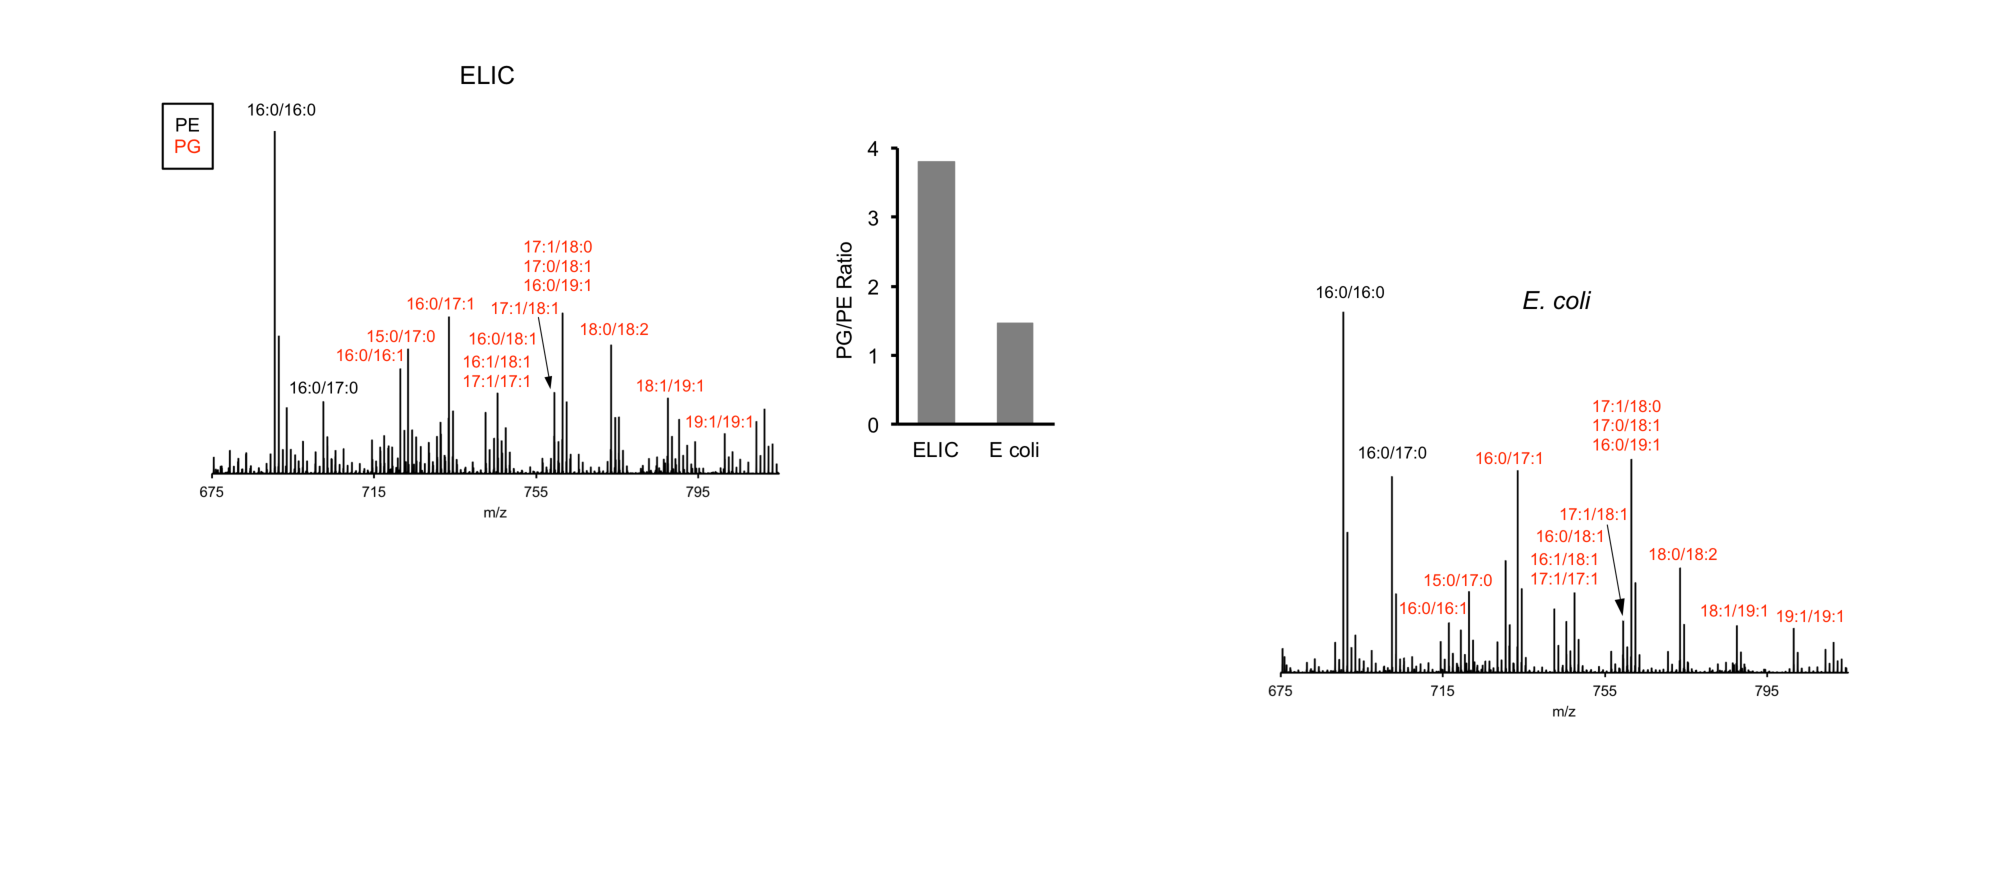
\includegraphics[width=5.95065in,height=3.02741in]{./pandoc_test/media/image11.pdf}
%
%\textbf{Supplementary Fig 1.} MS1 spectra of lipid extract from purified
%ELIC in DDM and \emph{E. coli} membranes. Labeled peaks correspond to PG
%(red) and PE (black) phospholipids with specific acyl chain combinations
%determined from MS2 fragmentation. \emph{Right:} Graph shows
%quantification of the intensity of all PG species relative to PE species
%for ELIC and \emph{E. coli} membrane samples.
%
%\textbf{\\
%}
%
%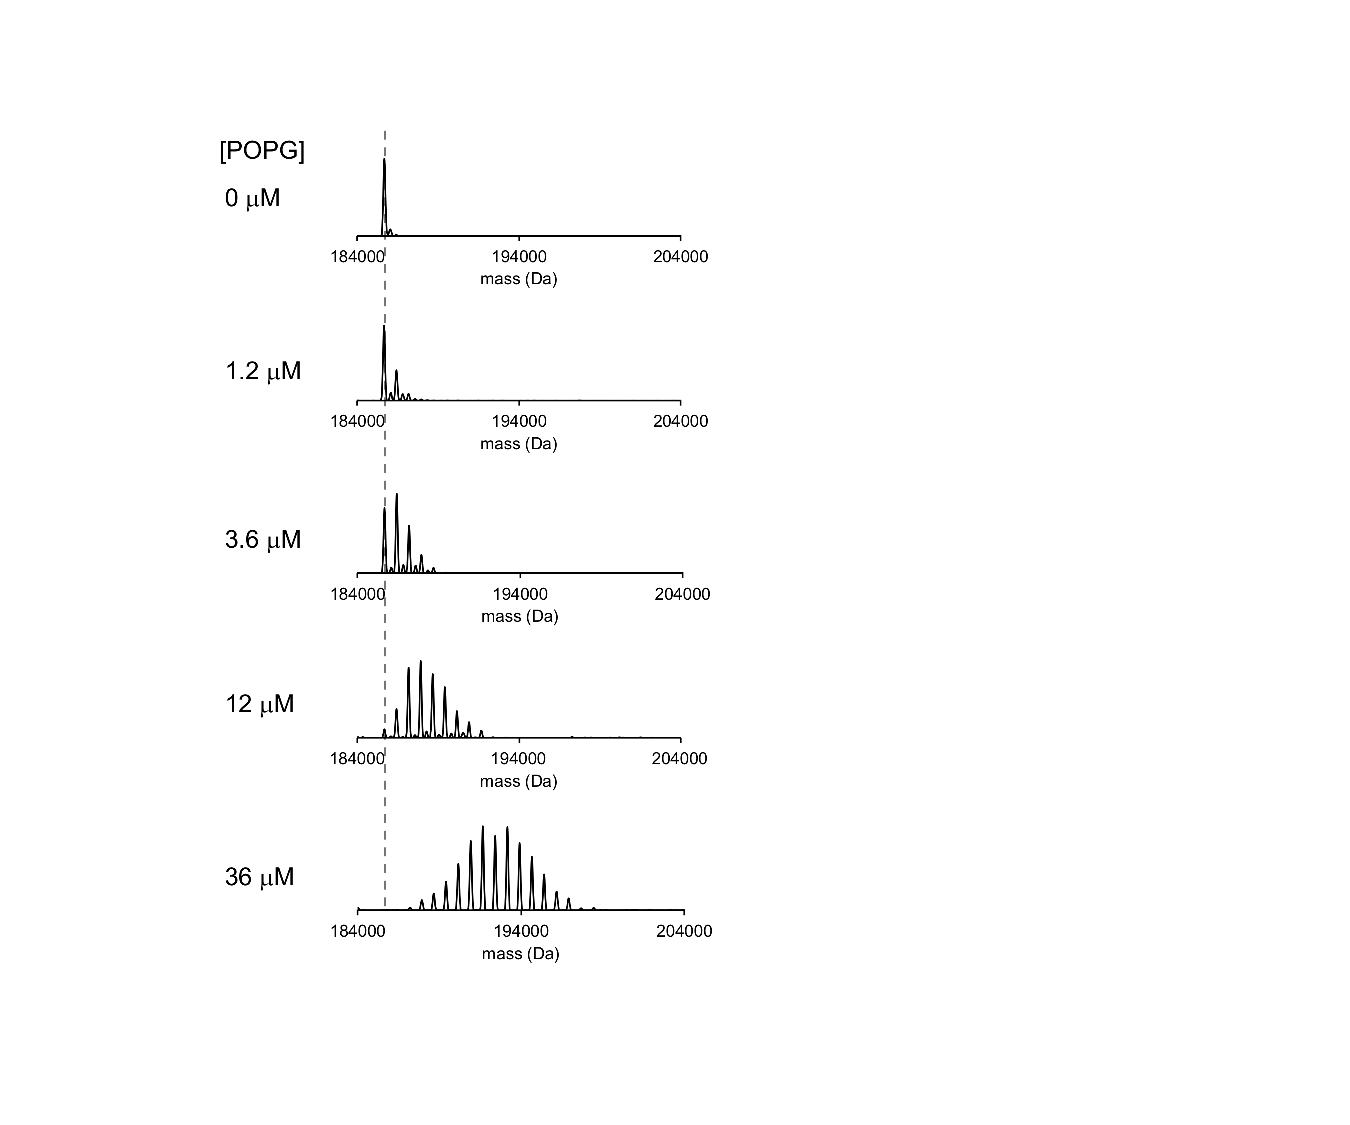
\includegraphics[width=3.18125in,height=5.31611in]{./pandoc_test/media/image12.pdf}
%
%\textbf{Supplementary Fig. \ref{fig:two}.} Representative deconvoluted spectra of 1
%$\mu$M ELIC in C10E5 with increasing concentration of POPG. Dashed line
%indicates mass of apo ELIC.
%
%\textbf{\\
%}
%
%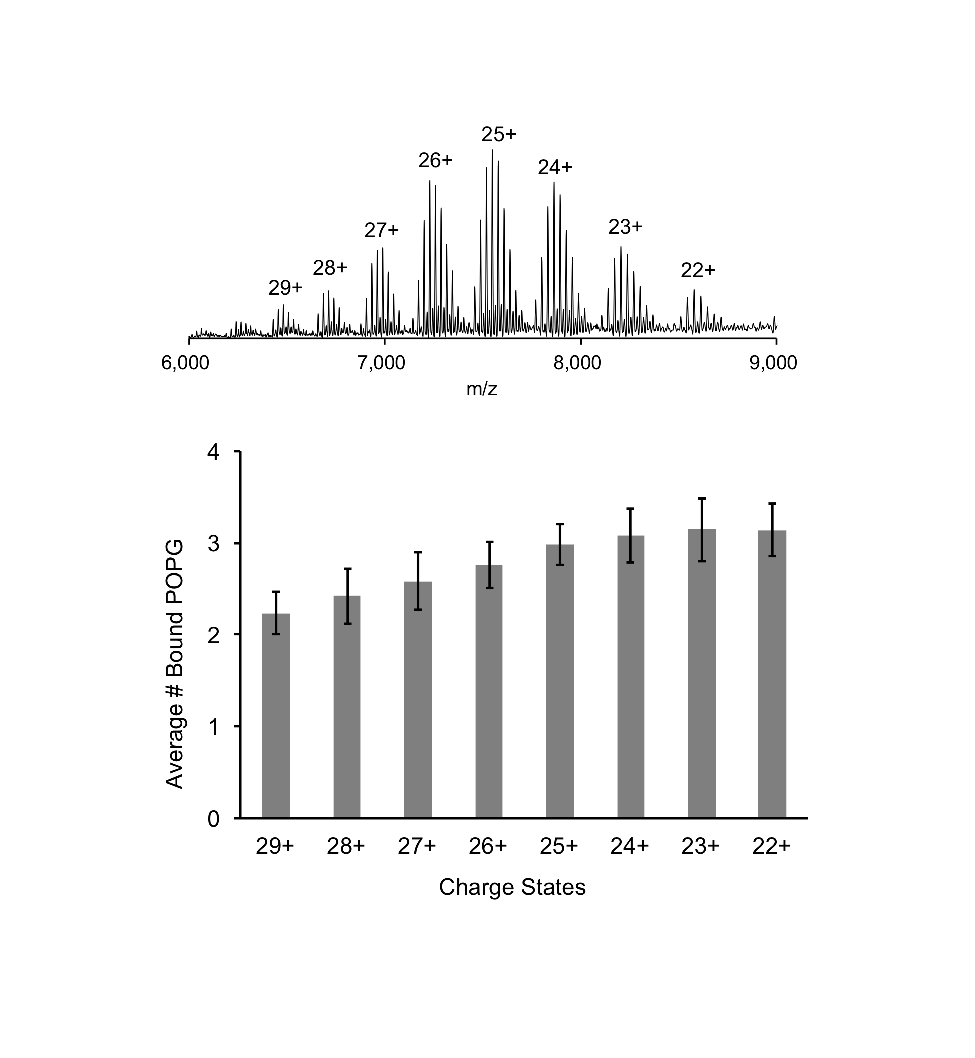
\includegraphics[width=4.64167in,height=5.34307in]{./pandoc_test/media/image13.pdf}
%
%\textbf{Fig. \ref{fig:Supplementary Table 3}.} Comparison of lipid binding at different
%charge states. \emph{Top:} Representative full native spectrum of the
%ELIC pentamer with 12 $\mu$M POPG with each charge state labeled.
%\emph{Bottom:} Quantification of the average number of bound POPG to the
%ELIC pentamer at each charge state (n=13, $\pm$SD).
%
%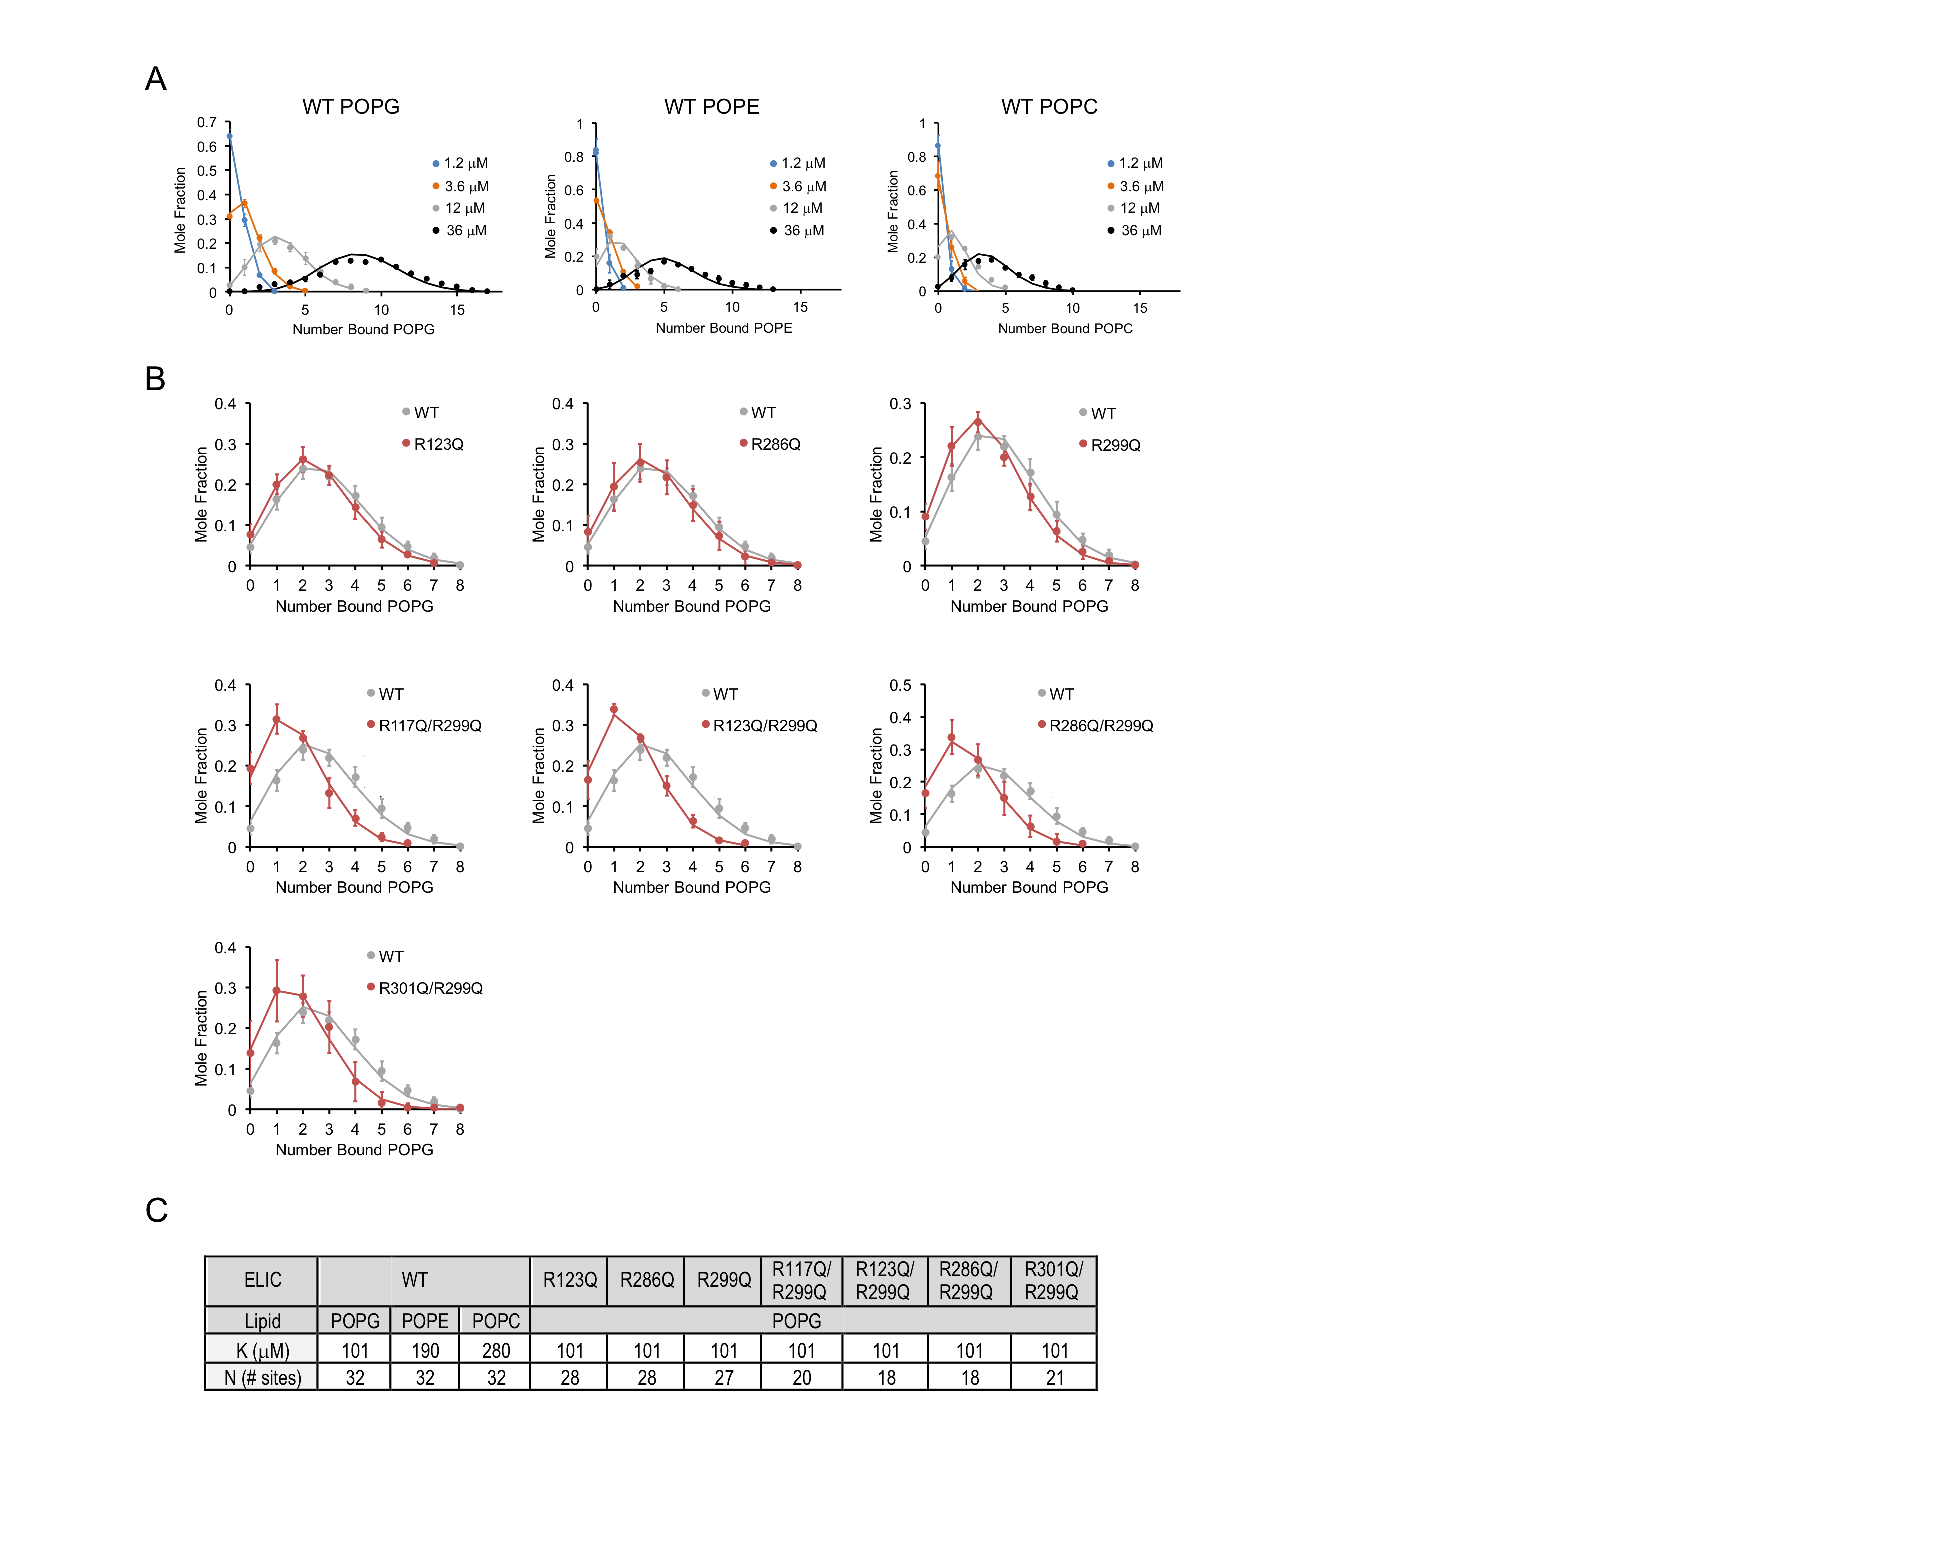
\includegraphics[width=5.51458in,height=7.04808in]{./pandoc_test/media/image14.pdf}
%
%\textbf{Supplementary Fig. \ref{fig:six}.} Lipid binding data fit to binomial
%distributions. (\textbf{A}) Plots of mole fraction of phospholipid-bound
%ELIC derived from native MS experiments with varying concentrations of
%phospholipid (circles, n=3-6, $\pm$SD). Solid lines show global fits from a
%binding model based on a binomial distribution with 32 sites (N) of
%equal affinity (K) using K as shown in (C). (\textbf{B}) Plots of mole
%fraction of POPG-bound ELIC WT and mutants at 12 $\mu$M POPG (circles,
%n=3-6, $\pm$SD). Solid lines show fits as in (A) in which K is held constant
%at 102 $\mu$M and N is varied as indicated in (C). (\textbf{C}) Table
%showing dissociation constants (K) and number of sites (N) used in fits
%shown in (A) and (B).
%
%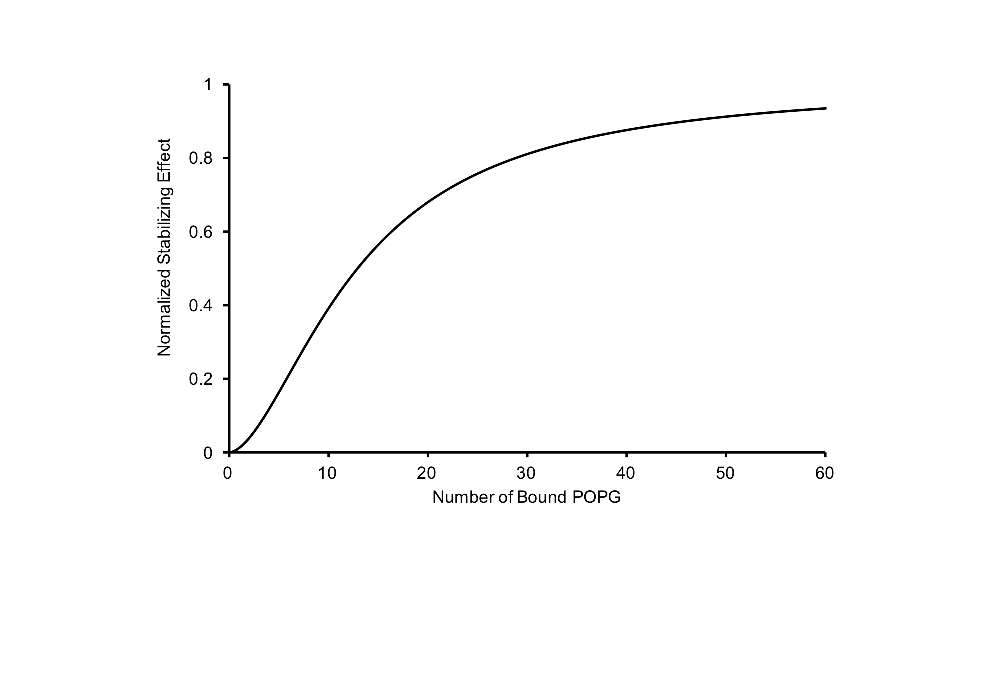
\includegraphics[width=3.93125in,height=2.48554in]{./pandoc_test/media/image15.pdf}
%
%\textbf{Supplementary Fig. \ref{fig:seven}.} Relationship of the thermal stabilizing
%effect of POPG vs the average number of bound POPG derived from equating
%concentration of POPG from the sigmoid functions used to fit the POPG
%binding (Fig. \ref{fig:one}B) and thermal stability data (Fig. \ref{fig:two}A). The resulting
%relationship is: \(S = \ \frac{1}{1 + {(\frac{13.7}{P)}}^{1.7}}\) ,
%where P is the average number of bound POPG and S is the normalized
%thermal stabilizing effect.
%
%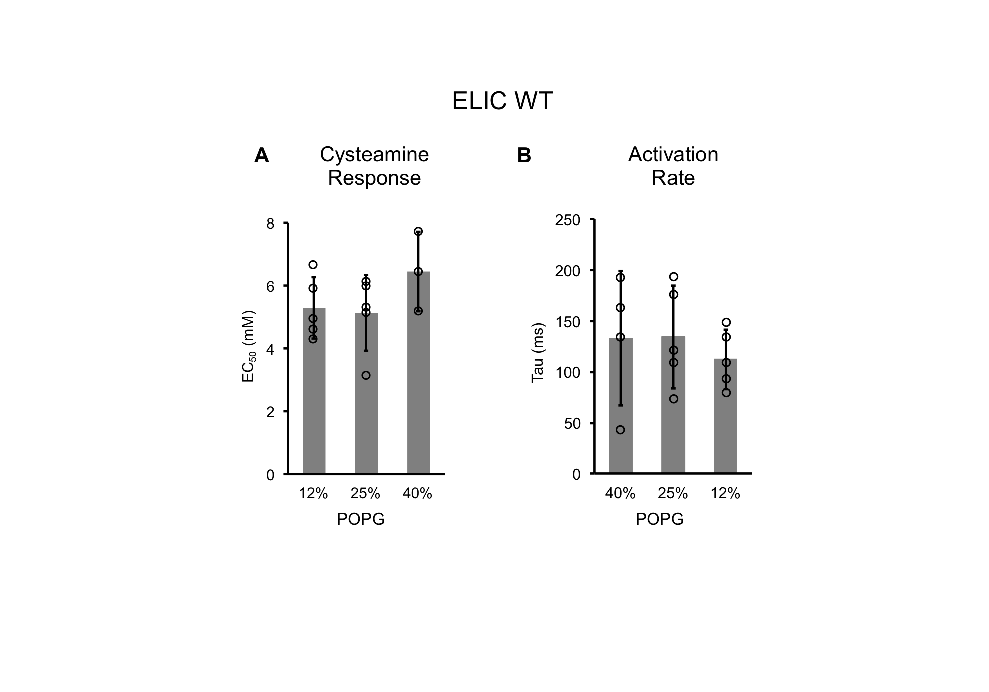
\includegraphics[width=3.67880in,height=3.12778in]{./pandoc_test/media/image16.pdf}
%
%\textbf{Supplementary Fig. \ref{fig:eight}.} Channel properties of WT ELIC responses
%to cysteamine. (\textbf{A}) EC\textsubscript{50} for peak responses to
%cysteamine of WT ELIC in giant liposomes of varying mole\% POPG (n=3-5,
%$\pm$SD). (\textbf{B}) Activation time constants ($\tau$) derived from single
%exponential fits of WT ELIC in response to 30 mM cysteamine in giant
%liposomes of varying mole\% POPG (n=4-5, $\pm$SD).
%
%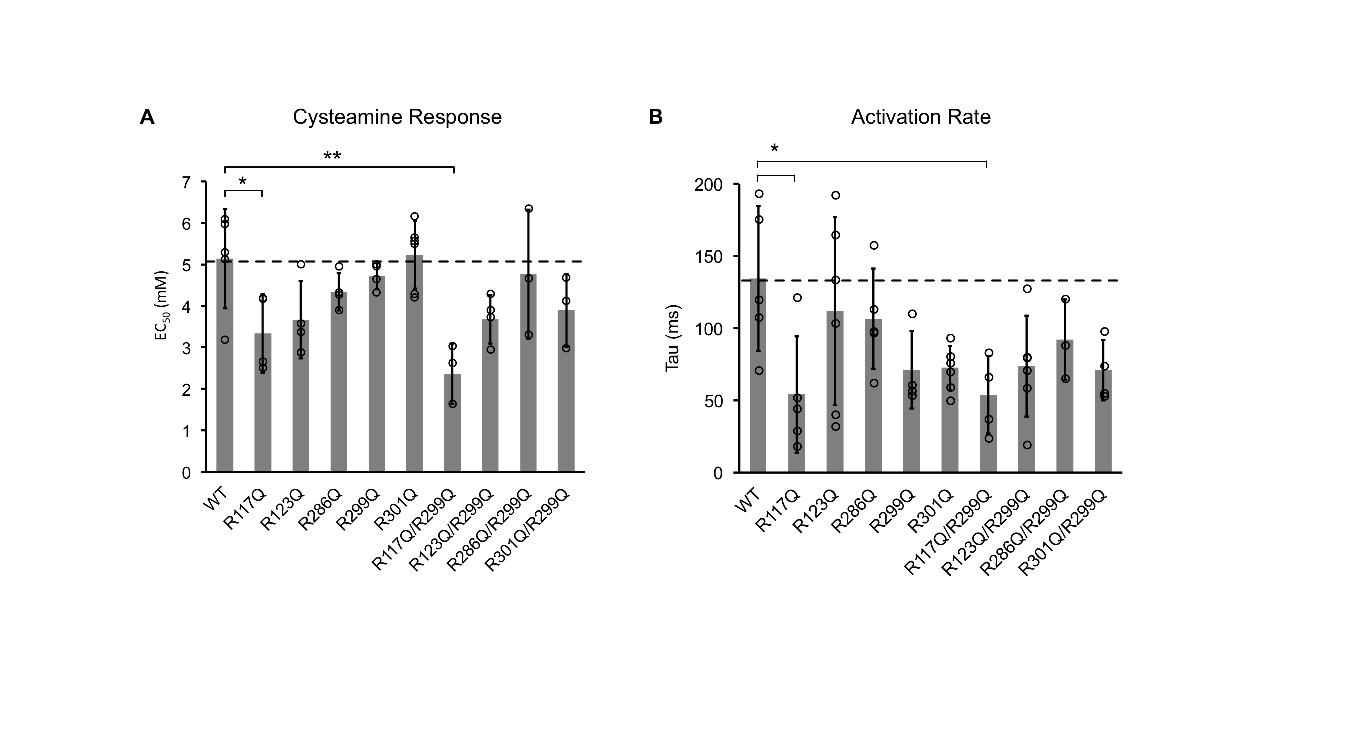
\includegraphics[width=6.43181in,height=3.12778in]{./pandoc_test/media/image17.pdf}
%
%\textbf{Supplementary Fig. \ref{fig:ten}.} Channel properties of ELIC WT and mutant
%responses to cysteamine in giant liposomes of 25 mole\% POPG.
%(\textbf{A}) Graph of EC\textsubscript{50} for peak responses to
%cysteamine of ELIC WT and mutants (n=4-7, $\pm$SD, *p\textless{}0.05,
%**p\textless{}0.01). (\textbf{B}) Activation time constants (tau) of
%ELIC WT and mutants in response to 30 mM cysteamine (n=4-7, $\pm$SD,
%**p\textless{}0.01).
%
%\end{document}
